\documentclass[conference]{IEEEtran}
\IEEEoverridecommandlockouts
% The preceding line is only needed to identify funding in the first footnote. If that is unneeded, please comment it out.
\usepackage{cite}
\usepackage{amsmath,amssymb,amsfonts}
\usepackage{float}
\usepackage{algorithmic}
\usepackage{graphicx}
\usepackage{enumitem}
\usepackage{textcomp}
\usepackage{xcolor}
\usepackage{hyperref}
\def\BibTeX{{\rm B\kern-.05em{\sc i\kern-.025em b}\kern-.08em
    T\kern-.1667em\lower.7ex\hbox{E}\kern-.125emX}}
    \pagestyle{plain}

\begin{document}

\title{Detecting Coral Eating Crown Of Thorns Starfish with YOLOv8}

\author{\IEEEauthorblockN{Vikas Kumar}
\IEEEauthorblockA{\textit{110156183} \\
\textit{University of Windsor}\\
Windsor, Canada \\
kumar3s@uwindsor.ca}
}

\maketitle

\begin{abstract}
The Great Barrier Reef, one of the world's most diverse marine ecosystems, faces significant threats due to the overpopulation of the coral-eating crown-of-thorns starfish (COTS). Current monitoring methods, such as the "Manta Tow" survey, are limited in scalability, data resolution, and reliability. To address these challenges, this research focuses on developing a real-time object detection model using neural networks and deep learning techniques to identify COTS from underwater videos of coral reefs.

Leveraging video datasets provided by Australia’s national science agency (CSIRO\cite{csiro}) and Google, the study employs advanced machine learning architectures to enhance the detection accuracy and efficiency of underwater species monitoring. The proposed model incorporates convolutional neural networks (CNNs) for feature extraction and advanced object detection algorithms such as YOLOv8 to achieve high-resolution, real-time performance. The methodology includes rigorous data preprocessing, augmentation, and iterative model training to optimize performance under challenging underwater conditions, including poor lighting and occlusion.

This research contributes to scalable, precise, and actionable monitoring solutions by automating COTS detection, empowering researchers and reef managers to manage outbreaks better and protect the reef ecosystem. The outcomes are expected to assist in AI-driven environmental conservation, providing a robust framework for future applications in marine biodiversity monitoring.
\end{abstract}

\begin{IEEEkeywords}
Object Detection, Deeplearning Learning, Convolutional Neural Networks, video frames, YOLO
\end{IEEEkeywords}

% ======================
% ======================
% Introduction
% ======================
% ======================

\section{Introduction}
The Great Barrier Reef, a UNESCO World Heritage Site, is under significant ecological threat due to the overpopulation of the COTS. These coral-eating starfish contribute to coral degradation, necessitating efficient monitoring and control measures. Traditional reef survey methods, such as "Manta Tow," have proven effective but are constrained by scalability, data resolution, and reliability issues. To address these challenges, this project tries to focus on leveraging neural networks and deep learning techniques to develop an automated object detection system for identifying COTS in underwater videos.

\subsection{Purpose of the Project}
The primary purpose of this project is to create an object detection model capable of real-time identification of COTS in underwater videos. This solution aims to assist researchers and conservationists in monitoring and mitigating COTS outbreaks, contributing to the preservation of the Great Barrier Reef.

\subsection{Problem Statement}
Current methods of monitoring COTS, including manual surveys and visual assessments, are labor-intensive, time-consuming, and prone to errors. These limitations hinder large-scale implementation and timely intervention. Developing an AI-based solution for automated detection and monitoring of COTS offers a scalable and efficient alternative.

\subsection{Motivation}
Preserving the biodiversity and ecological health of the Great Barrier Reef is critical for marine life and global environmental sustainability. This project aims to empower conservationists with tools that enhance the accuracy and efficiency of monitoring efforts by advancing machine learning technologies for marine conservation.

\subsection{Aim}
This study aims to build an object detection system using neural networks and deep learning to detect COTS in underwater videos with high accuracy and efficiency.

\subsection{Objectives}
\begin{itemize}
    \item To preprocess and annotate underwater video data for optimal input into deep learning models.
    \item To develop a neural network-based object detection algorithm that is optimized for underwater conditions, including varying lighting and visibility.
    \item To evaluate the model's performance against key metrics such as precision, recall, and inference time.
\end{itemize}

\subsection{Approach}
This project employs a deep learning approach using convolutional neural networks (CNNs) and the object detection model YOLOv8. The project involves data preprocessing, visualizing, augmenting, testing various hyper-parameters, and training the model.
\begin{enumerate}
    \item Identify the best size of model for our project.
    \item Figure out techniques to train the model on our data.
    \item Training and fine-tuning the detection model on annotated datasets.
    \item Testing and evaluating the model's performance on the test dataset.
\end{enumerate}

\subsection{Experimental Setup and Demonstration}
The experimental setup involves:
\begin{itemize}
    \item A curated dataset from underwater video footage of the Great Barrier Reef, divided into training and test sets.
    \item Python to interact with the pre-trained YOLOV8 models
    \item A CUDA-enabled computing environment with GPU acceleration for efficient training of deep learning models.
    \item The final output includes a submission file demonstrating the model's predictions on the test dataset.
\end{itemize}

\subsection{System Workflow}
The system workflow comprises the following steps:
\begin{enumerate}
    \item \textbf{Data Acquisition \& Annotation:} The CSIRO dataset\cite{liu2021csiro} contains frames of 3 videos taken through the Manta Tow method and all the COTS were labeled manually.
    \item \textbf{Model Training:} Training the object detection model using annotated data, leveraging transfer learning for better results.
    \item \textbf{Evaluation:} Validating model performance using metrics such as mean Average Precision (mAP) and assessing real-time inference capabilities.
\end{enumerate}

% ======================
% ======================
% Existing Work
% ======================
% ======================
\section{Existing Work}
The CSIRO Crown-of-Thorns Starfish Detection Dataset provides a comprehensive, annotated collection of underwater images for object detection research. The dataset was developed to address the ecological challenges posed by COTS outbreaks on the Great Barrier Reef (GBR), which are a major cause of COTS loss. Below, we outline the key aspects of this dataset and its significance in advancing research on machine learning-driven environmental monitoring.

\subsection{Data Collection Methodology}
The dataset was meticulously gathered using GoPro Hero9 cameras integrated with the traditional Manta Tow method. The cameras were attached to the bottom of the tow boards held by snorkeler-divers during underwater surveys. This setup allowed the recording of oblique views of the reef at various depths and distances. The snorkelers were towed behind a boat moving at speeds of up to 5 knots for transects approximately 200 meters long. Videos were recorded continuously at a resolution of 3840x2160 pixels and 24 frames per second. To ensure the dataset's quality and focus, periods of inactivity between transects were manually removed.

The collected footage underwent an AI-assisted annotation process, where pre-trained COTS detection models assisted expert annotators in identifying and marking instances of COTS using bounding boxes. This collaboration between domain experts and machine learning technologies resulted in a high-quality, validated dataset with annotations tailored for object detection.

\subsection{Existing Methods for Data Collection}
Traditionally, monitoring COTS populations has relied on the Manta Tow method, where snorkeler-divers visually assess underwater habitats and manually record observations after each transect. While effective for general surveys, this method has limitations in terms of scalability, data resolution, and reliability. The integration of underwater imaging and AI models addresses these shortcomings, enabling large-scale, automated, and high-resolution monitoring of reef habitats.

\subsection{Advancements and Contributions}
The CSIRO dataset is significant for several reasons:
\begin{itemize}
    \item \textbf{Scalability and Precision:} The use of AI models in annotating and analyzing underwater images allows for broader and more accurate surveys compared to manual observation.
    \item \textbf{Dataset Characteristics:} Unlike conventional object detection datasets, this collection focuses on a single class (COTS), includes overlapping and partially visible objects, and provides sequential image data for enhanced analysis.
    \item \textbf{Ecological Impact:} By facilitating more efficient monitoring of COTS outbreaks, the dataset supports efforts to maintain the ecological balance of the GBR and mitigate the damage caused by these outbreaks.
\end{itemize}

This dataset represents a critical step in leveraging AI for environmental challenges, demonstrating how technology can complement traditional ecological practices. Its release through platforms like Kaggle further promotes collaboration within the machine learning community, fostering advancements in both environmental science and AI methodologies.




% ======================
% ======================
% Proposed Model
% ======================
% ======================

\section{Proposed Model}
YOLOv8, the 8th iteration in the You Only Look Once (YOLO) series, represented a significant advancement in real-time object detection technology. Developed by the Ultralytics team\cite{ultralytics2023yolov8explained}, YOLOv8 builds upon the success of its predecessors, introducing architectural innovations that enhance accuracy and efficiency for a wide range of applications.
\begin{figure}[H]
    \centering
    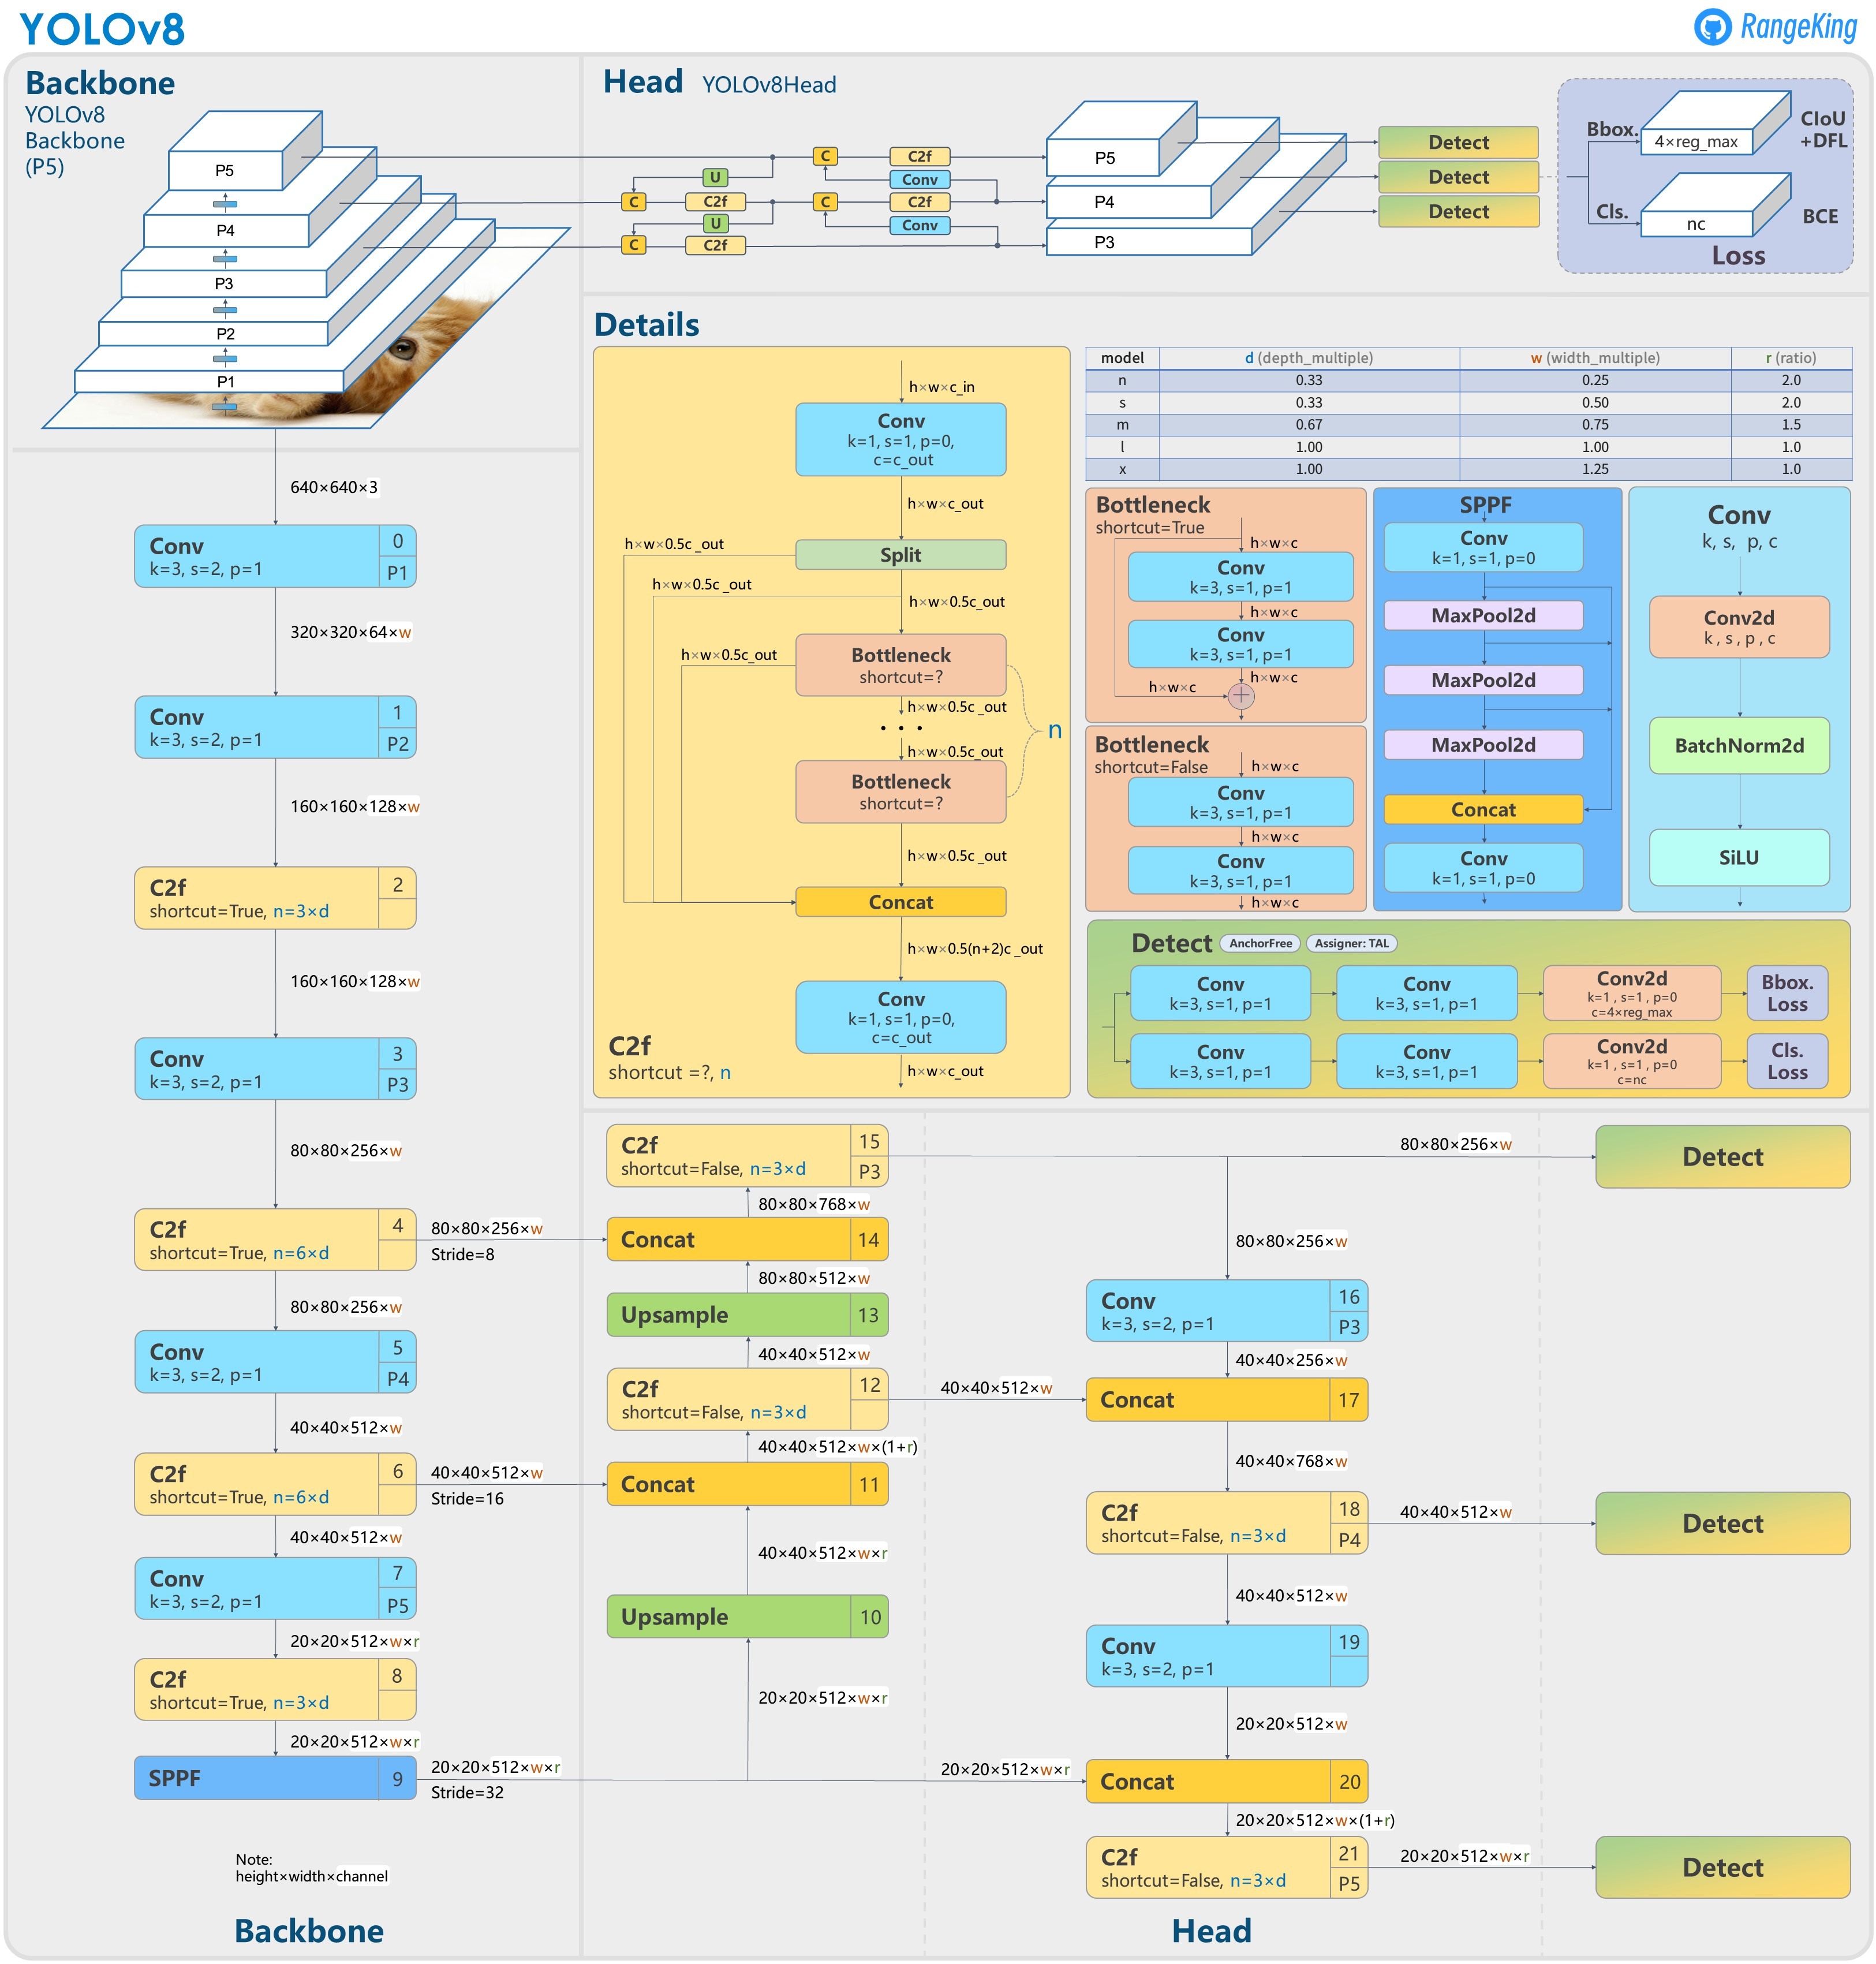
\includegraphics[width=0.5\textwidth]{yolov8-arch.jpg} 
    \caption{YOLO V8 architecture\cite{ultralytics2023yolov8} }
    \label{fig:metadata-schema}
\end{figure}
\subsection{Overview of YOLOv8 Architecture}
YOLOv8’s architecture is divided into three main components:
\begin{itemize}
    \item \textbf{Backbone:} The backbone, built on CSPDarknet53, extracts features from input images using cross-stage partial (CSP) connections. These connections improve information flow and gradient propagation, enhancing accuracy and computational efficiency.
    \item \textbf{Neck:} YOLOv8 employs a novel C2f module as its neck, replacing the traditional Feature Pyramid Network (FPN). This module fuses low-level spatial features with high-level semantic features, significantly improving detection accuracy, particularly for small objects.
    \item \textbf{Head:} The head is designed for predictions, integrating dynamic anchor assignment and an enhanced Intersection over Union (IoU) loss function. This design improves the accuracy of bounding box predictions and object classification.
\end{itemize}

\subsection{Key Innovations in YOLOv8}
YOLOv8 introduces several advancements that set it apart from earlier YOLO models:
\begin{itemize}
    \item \textbf{Spatial Attention:} A mechanism that emphasizes important areas in the image, enhancing object localization.
    \item \textbf{Feature Fusion:} The C2f module improves the combination of features across different scales.
    \item \textbf{Bottlenecks and SPPF:} The Spatial Pyramid Pooling Fast (SPPF) layer captures multi-scale features efficiently, while bottlenecks reduce computational complexity.
    \item \textbf{Data Augmentation:} Techniques like mosaic augmentation improve generalization, and mixed precision training speeds up model training without compromising performance.
\end{itemize}

\subsection{Benefits of YOLOv8}
YOLOv8 offers several notable benefits:
\begin{itemize}
    \item \textbf{High Accuracy:} State-of-the-art accuracy on benchmarks like COCO and VOC datasets.
    \item \textbf{Real-time Speed:} Optimized for fast inference, YOLOv8 is suitable for time-sensitive applications like robotics and autonomous vehicles.
    \item \textbf{Efficiency:} Lightweight design allows deployment on edge devices with limited computational power.
    \item \textbf{Open Source:} YOLOv8 is supported by a strong open-source community, fostering collaboration and continuous improvement.
\end{itemize}

\subsection{YOLOv8 Performance Metrics and Model Variants}
YOLOv8 demonstrates state-of-the-art performance in terms of mean Average Precision (mAP) and processing speeds on benchmark datasets. The model offers different configurations tailored to various use cases:
\begin{itemize}
    \item \textbf{YOLOv8-C:} Lightweight version for fast inference on edge devices.
    \item \textbf{YOLOv8-D:} Default configuration balancing accuracy and speed.
    \item \textbf{YOLOv8-E:} Enhanced version for high-accuracy tasks requiring greater computational resources.
\end{itemize}

\subsection{Comparison with Other Models}
Compared to other state-of-the-art models, YOLOv8 achieves a remarkable balance between speed and accuracy. Its anchor-free detection head and optimized loss function make it particularly suitable for real-time applications. With an easy-to-use API and robust documentation, YOLOv8 is an appealing choice for researchers and practitioners alike.

YOLOv8 exemplifies the ongoing evolution of object detection algorithms, combining high accuracy, real-time speed, and computational efficiency. Its innovative architecture and training strategies make it a versatile and powerful tool for applications ranging from autonomous vehicles to medical imaging. As research in this domain progresses, YOLOv8 serves as a benchmark for future developments in object detection.
\subsection{Explanation of the Model}
c2f, details about yolo components, from a math point of view

\subsection{Workflow Overview}


\subsection{Workflow Diagram Explanation}


\subsection{Differences from Existing Works}
Our model differs by providing:



% ======================
% ======================
% Methodology
% ======================
% ======================
\section{Methodology}

This study employed a comprehensive approach to train an object detection model for COTS detection using the YOLOv8 architecture. The methodology was designed to address the challenges posed by underwater environments, including varying lighting conditions, object occlusions, and motion distortions. Key aspects of the methodology involved data augmentation techniques and hyperparameter tuning, which were systematically explored to optimize the training process.

\subsection{Augmentation Techniques}

Data augmentation is a vital step in preparing a training dataset for robust model performance. It involves applying transformations to simulate various real-world scenarios, thereby expanding the effective size of the dataset and enhancing the model's generalization capabilities. For this study, multiple augmentation techniques were considered, which can be broadly categorized as follows:

\subsubsection{Color and Lighting Transformations}

Adjustments in hue, saturation, and brightness were applied to account for variations in lighting and visibility, simulating conditions caused by depth, turbidity, or refracted light in underwater environments.

\begin{enumerate}
    \item \textbf{Hue Adjustment}:
    \[
    I'_{\text{hue}} = (I_{\text{hue}} + \Delta h) \mod 360
    \]
    where \( I_{\text{hue}} \) is the original hue value of a pixel, and \( \Delta h \) is the hue shift in degrees.

    \item \textbf{Saturation Adjustment}:
    \[
    I'_{\text{sat}} = \min(I_{\text{sat}} \times s, 1.0)
    \]
    where \( I_{\text{sat}} \) is the original saturation, and \( s \) is the saturation scaling factor.

    \item \textbf{Brightness Adjustment}:
    \[
    I'_{\text{bright}} = I_{\text{bright}} + \beta
    \]
    where \( I_{\text{bright}} \) is the original brightness, and \( \beta \) is the brightness shift.
\end{enumerate}

These transformations help the model learn under different lighting conditions, improving its robustness to environmental variations.

\subsubsection{Geometric Transformations}

Geometric augmentations were applied to create diversity in object positioning and orientation, ensuring the model's robustness to different viewing angles and scales.

\begin{enumerate}
    \item \textbf{Rotation}:
    \[
    \begin{bmatrix}
    x' \\ y'
    \end{bmatrix}
    =
    \begin{bmatrix}
    \cos \theta & -\sin \theta \\
    \sin \theta & \cos \theta
    \end{bmatrix}
    \begin{bmatrix}
    x \\ y
    \end{bmatrix}
    \]
    where \( \theta \) is the rotation angle in radians.

    \item \textbf{Translation}:
    \[
    \begin{bmatrix}
    x' \\ y'
    \end{bmatrix}
    =
    \begin{bmatrix}
    x + \Delta x \\ y + \Delta y
    \end{bmatrix}
    \]
    where \( \Delta x \) and \( \Delta y \) are the translation offsets.

    \item \textbf{Scaling}:
    \[
    \begin{bmatrix}
    x' \\ y'
    \end{bmatrix}
    = s
    \begin{bmatrix}
    x \\ y
    \end{bmatrix}
    \]
    where \( s \) is the scaling factor.

    \item \textbf{Shearing}:
    \[
    \begin{bmatrix}
    x' \\ y'
    \end{bmatrix}
    =
    \begin{bmatrix}
    1 & m_x \\
    m_y & 1
    \end{bmatrix}
    \begin{bmatrix}
    x \\ y
    \end{bmatrix}
    \]
    where \( m_x \) and \( m_y \) are shear coefficients along the \( x \)- and \( y \)-axes, respectively.
\end{enumerate}

By applying these transformations, the model becomes invariant to object orientation and position, improving detection accuracy in real-world scenarios.

\subsubsection{Perspective Distortion}

Perspective transformations were introduced to simulate viewing objects from different angles or through refractive media like water.

\[
\begin{bmatrix}
x' \\ y' \\ w
\end{bmatrix}
=
\begin{bmatrix}
h_{11} & h_{12} & h_{13} \\
h_{21} & h_{22} & h_{23} \\
h_{31} & h_{32} & h_{33}
\end{bmatrix}
\begin{bmatrix}
x \\ y \\ 1
\end{bmatrix}
\]
The transformed coordinates are obtained by normalizing:
\[
x'' = \frac{x'}{w}, \quad y'' = \frac{y'}{w}
\]
where \( h_{ij} \) are elements of the homography matrix \( \mathbf{H} \).

This augmentation helps the model handle distortions caused by camera angles and water refraction.

\subsubsection{Flipping}

Vertical and horizontal flips were used to create variability in object orientation.

\begin{enumerate}
    \item \textbf{Horizontal Flip}:
    \[
    x' = W - x
    \]
    \item \textbf{Vertical Flip}:
    \[
    y' = H - y
    \]
\end{enumerate}
where \( W \) and \( H \) are the image width and height, respectively.

Flipping increases data diversity, allowing the model to generalize better to different orientations.

\subsubsection{Advanced Augmentations}

\begin{enumerate}
    \item \textbf{Mosaic Augmentation}:
    Combines four different images into one large image, placing them in a 2x2 grid. This exposes the model to more context and object scales within a single training sample.

    \item \textbf{Mixup Augmentation}:
    Blends two images and their corresponding labels:
    \[
    I_{\text{mix}} = \lambda I_1 + (1 - \lambda) I_2
    \]
    \[
    y_{\text{mix}} = \lambda y_1 + (1 - \lambda) y_2
    \]
    where \( \lambda \sim \text{Beta}(\alpha, \alpha) \) and \( \alpha \) is a hyperparameter.

    \item \textbf{Occlusion Simulation (Random Erasing)}:
    Randomly selects a rectangular region in an image and erases its pixels:
    \[
    I'(x, y) =
    \begin{cases}
    I(x, y), & \text{if } (x, y) \notin \text{erased region} \\
    0, & \text{if } (x, y) \in \text{erased region}
    \end{cases}
    \]

    \item \textbf{Auto-Augmentation}:
    Automated strategies like RandAugment dynamically apply a range of transformations without manual selection:
    \[
    \text{Augment}_{\text{auto}} = \text{RandomChoice}(\text{Transformations})
    \]
\end{enumerate}

These advanced augmentations encourage the model to generalize better and reduce overfitting by exposing it to a wider range of variations.

\subsubsection{Impact on Training Process}

The selected augmentation techniques offered unique benefits to the training process, balancing simplicity with effectiveness. They enhanced the diversity of the training data, enabling the model to generalize to diverse and challenging underwater conditions, such as varying lighting, object orientations, and occlusions.

\subsection{Hyperparameter Tuning}

Hyperparameter tuning is crucial for optimizing the training process and enhancing the model's generalization ability. The following key hyperparameters and their configurations were explored:

\subsubsection{Learning Rate}

The learning rate (\( \eta \)) controls the magnitude of weight updates during training.

\begin{enumerate}
    \item \textbf{Fixed Learning Rate}:
    \[
    \eta_t = \eta_0
    \]

    \item \textbf{Decay-Based Schedules}:
    \[
    \eta_t = \eta_0 \times \gamma^{\left\lfloor \frac{t}{T_{\text{decay}}} \right\rfloor}
    \]
    where \( \gamma \) is the decay rate, \( t \) is the current epoch, and \( T_{\text{decay}} \) is the decay step.

    \item \textbf{Cosine Annealing}:
    \[
    \eta_t = \eta_{\text{min}} + \frac{1}{2} (\eta_{\text{max}} - \eta_{\text{min}}) \left(1 + \cos\left( \frac{t}{T} \pi \right)\right)
    \]
\end{enumerate}

An adaptive schedule like cosine annealing allows the learning rate to adjust dynamically, facilitating better convergence.

\subsubsection{Batch Size}

Batch size (\( B \)) defines the number of samples processed together during training.

\[
\theta_{t+1} = \theta_t - \frac{\eta_t}{B} \sum_{i=1}^{B} \nabla_\theta L(f(x_i; \theta_t), y_i)
\]
where \( L \) is the loss function, \( \theta \) are the model parameters, and \( (x_i, y_i) \) are the training samples and labels.

A batch size of 32 was chosen to balance computational efficiency and gradient stability.

\subsubsection{Optimizer Choices}

Optimizers update model weights to minimize the loss function.

\begin{enumerate}
    \item \textbf{AdamW}:
    \[
    m_t = \beta_1 m_{t-1} + (1 - \beta_1) \nabla_\theta L_t
    \]
    \[
    v_t = \beta_2 v_{t-1} + (1 - \beta_2) (\nabla_\theta L_t)^2
    \]
    \[
    \hat{m}_t = \frac{m_t}{1 - \beta_1^t}
    \]
    \[
    \hat{v}_t = \frac{v_t}{1 - \beta_2^t}
    \]
    \[
    \theta_{t+1} = \theta_t - \eta_t \frac{\hat{m}_t}{\sqrt{\hat{v}_t} + \epsilon} - \eta_t \lambda \theta_t
    \]
    where \( \beta_1 \) and \( \beta_2 \) are momentum terms, and \( \lambda \) is the weight decay coefficient.

    AdamW was selected for its adaptive learning rates and effective regularization, making it suitable for complex tasks.
\end{enumerate}

\subsubsection{Regularization}

Regularization techniques prevent overfitting by penalizing complex models.

\begin{enumerate}
    \item \textbf{Weight Decay}:
    Adds an \( L_2 \) penalty to the loss function:
    \[
    L_{\text{total}} = L_{\text{data}} + \lambda ||\theta||_2^2
    \]
    where \( \lambda \) is the regularization parameter.

    \item \textbf{Augmentation-Driven Regularization}:
    Data augmentation inherently acts as regularization by increasing data diversity.
\end{enumerate}

\subsubsection{Warmup Strategies}

Warmup phases gradually increase the learning rate at the start of training.

\begin{enumerate}
    \item \textbf{Linear Warmup}:
    \[
    \eta_t = \eta_{\text{max}} \times \frac{t}{T_{\text{warmup}}}, \quad t \leq T_{\text{warmup}}
    \]
    where \( T_{\text{warmup}} \) is the number of warmup epochs.
\end{enumerate}

Warmup helps stabilize early training by preventing large gradient updates that could disrupt convergence.

\subsubsection{Early Stopping}

Early stopping monitors validation performance and halts training when improvements plateau, preventing overfitting.

If the validation loss does not improve for \( P \) consecutive epochs (patience), training is stopped.

\subsubsection{Confidence Threshold}

The confidence threshold (\( \tau \)) filters predictions based on their probability scores.

\[
\text{Prediction} = 
\begin{cases}
\text{Positive}, & \text{if } P(\text{object}) > \tau \\
\text{Negative}, & \text{otherwise}
\end{cases}
\]

Lower thresholds increase recall but may include more false positives, while higher thresholds improve precision at the cost of recall.

\subsubsection{Impact on Training Process}

Each hyperparameter offered multiple configurations, and their effects were carefully evaluated through experimentation. The tuning process was guided by the goal of achieving an optimal balance between computational efficiency, precision, and recall while having more emphasis on recall compared to precision and ensuring that the model could adapt to the specific challenges of detecting COTS in underwater imagery.

\subsection{Summary}

By leveraging diverse augmentation techniques and systematically exploring hyperparameter configurations, this methodology aimed to build a robust and efficient object detection model. The variety of options allowed for flexibility in addressing specific challenges, while the tuning process ensured that the final model was well-suited for real-world applications in ecological monitoring. This approach underscores the importance of adaptability and experimentation in training high-performance models for complex tasks.



% ======================
% ======================
% Evaluation Method
% ======================
% ======================
\section{Evaluation Methods}

In this study, the performance of the object detection model was evaluated using a combination of widely adopted metrics that quantify the accuracy, recall, and overall effectiveness of detecting COTS in underwater imagery. These methods allow for a comprehensive assessment of the model's ability to identify and locate objects under varying conditions. Below is a detailed explanation of the key evaluation metrics and methods used in this research.

\subsection{Precision}
Precision is a critical metric in object detection, quantifying the model’s ability to make correct predictions. Specifically, it measures the proportion of predicted bounding boxes that are true positives (correctly detected COTS) out of all predicted bounding boxes. In other words, precision indicates how many of the model's detections were correct.

\begin{equation}
\text{Precision} = \frac{\text{True Positives (TP)}}{\text{True Positives (TP)} + \text{False Positives (FP)}}
\end{equation}

In the context of this study, high precision ensures that the model is accurately detecting COTS without many false detections. Given the nature of the COTS outbreak detection task, minimizing false positives is important to avoid misidentifications of other objects as COTS.

\subsection{Recall}
Recall measures the model’s ability to detect all relevant instances of COTS within an image, without missing any. Specifically, recall quantifies the proportion of ground truth bounding boxes (actual COTS) that are correctly identified by the model. High recall is crucial in this case, as the goal is to ensure that all visible COTS are detected, even if some might be partially obscured or overlapping.

\begin{equation}
\text{Recall} = \frac{\text{True Positives (TP)}}{\text{True Positives (TP)} + \text{False Negatives (FN)}}
\end{equation}

Given the ecological importance of detecting as many COTS as possible to manage the outbreaks, recall is prioritized over precision in this study. Missing even a few COTS could result in an incomplete survey, undermining control efforts.

\subsection{Intersection over Union (IoU)}
Intersection over Union (IoU) is a widely used metric in object detection that evaluates the overlap between the predicted bounding boxes and the ground truth bounding boxes. The IoU is calculated as:

\begin{equation}
IoU = \frac{\text{Area of Overlap}}{\text{Area of Union}}
\end{equation}

A predicted bounding box is considered a true positive (TP) if its IoU with the ground truth box exceeds a predefined threshold. In this study, different IoU thresholds were used, ranging from 0.50 to 0.95, to assess how well the model performs under different levels of detection accuracy. The stricter the threshold, the higher the overlap required for a prediction to be considered correct.

\subsection{Mean Average Precision (mAP)}
Mean Average Precision (mAP) is the primary metric for evaluating object detection models and is calculated based on the precision-recall curve at various thresholds. For this study, two variants of mAP were used:

\begin{itemize}
    \item \textbf{mAP50:} This is the average precision calculated at an IoU threshold of 0.50. It provides a relatively lenient evaluation, allowing for some discrepancies between predicted and ground truth boxes.
    \item \textbf{mAP50-95:} This variant calculates the average precision across multiple IoU thresholds (ranging from 0.50 to 0.95 in increments of 0.05), which is a more stringent and comprehensive measure.
\end{itemize}

The mAP metric is calculated by averaging the precision scores for COTS class over the all recall levels:

\begin{equation}
\text{mAP} = \frac{1}{N} \sum_{i=1}^{N} \text{AP}_i
\end{equation}

where $N$ is the number of IoU thresholds, and $\text{AP}_i$ is the average precision at the $i$-th threshold. This metric provides an overall indication of the model's ability to detect objects with varying degrees of overlap.

\subsection{Training Loss Metrics}
During the training process, several loss components were used to guide the optimization of the model. These losses were monitored for each epoch to track the model's learning progress:

\begin{itemize}
    \item \textbf{Box Loss:} This measures the error in predicting the coordinates of the bounding boxes relative to the ground truth. Lower box loss indicates that the model is accurately localizing COTS.
    \item \textbf{Class Loss:} This loss function measures the error in classifying the object within a predicted bounding box. It quantifies the discrepancy between the predicted class label and the true class label.
    \item \textbf{Distribution Focal Loss (DFL):} This loss function focuses on refining the localization of predicted bounding boxes by emphasizing more challenging or uncertain predictions, improving the precision of object localization.
\end{itemize}

These losses are essential for the model to converge and improve over time, adjusting its parameters to minimize errors in bounding box locations and classification.

\subsection{Epoch-Wise Evaluation}
After each epoch, the model's performance was validated on a held-out dataset, allowing the researchers to track improvements and diagnose potential overfitting or underfitting. The following metrics were reported at the end of each epoch:
\begin{itemize}
    \item Precision
    \item Recall
    \item mAP50 and mAP50-95
\end{itemize}

By evaluating these metrics after each epoch, we ensured that the model was improving its detection accuracy and reducing the loss values. This also allowed for fine-tuning hyperparameters and adjusting the training process as needed.


\subsection{Speed Metrics}
Inference speed is an important factor in evaluating the model's efficiency, especially in real-time applications. The following speed metrics were reported:
\begin{itemize}
    \item \textbf{Preprocessing Time:} The time spent on preparing input images for the model.
    \item \textbf{Inference Time:} The time the model takes to make predictions (i.e., detect objects).
    \item \textbf{Postprocessing Time:} The time spent on refining and formatting the outputs, such as applying non-maximum suppression (NMS) to filter redundant bounding boxes.
\end{itemize}

The reported average inference speed was approximately 14.4 milliseconds per image, which is fast enough for potential real-time monitoring of COTS outbreaks.

The evaluation methods used in this study provide a comprehensive and detailed assessment of the model's performance in detecting COTS in underwater imagery. By combining standard object detection metrics such as precision, recall, and mAP with training loss monitoring and speed evaluation, we ensured that the model was both accurate and efficient. These metrics align with the ecological objective of detecting as many COTS as possible, with minimal false positives, and provide insights into the model’s potential for real-time deployment in ecological monitoring systems.




% ======================
% ======================
% Results and Discussion
% ======================
% ======================
\section{Results and Discussion}
The experiments were run for three Yolo models small, medium, and large to check for overfitting, speed of inference, and ability to capture/understand necessary details.

\begin{table*}[t] % Use table* for spanning both columns
    \centering
    \caption{Summary of YOLOv8 Model Training Results for COTS Detection}
    \label{tab:training_results}
    \resizebox{\textwidth}{!}{% Automatically resize to fit the full page width
    \begin{tabular}{lcccccccc}
        \hline
        \textbf{Model} & \textbf{Layers} & \textbf{Parameters} & \textbf{GFLOPs} & \textbf{Precision} & \textbf{Recall} & \textbf{mAP50} & \textbf{mAP50-95} & \textbf{Inference Time (ms)} \\
        \hline
        YOLOv8s & 225 & 11,135,987 & 28.6 & 0.917 & 0.825 & 0.895 & 0.489 & 2.7 \\
        YOLOv8m & 295 & 25,856,899 & 79.1 & 0.912 & 0.805 & 0.873 & 0.465 & 5.6 \\
        YOLOv8l & 365 & 43,630,611 & 165.4 & 0.883 & 0.724 & 0.798 & 0.38  & 9.0 \\
        \hline
    \end{tabular}%
    }
\end{table*}


\subsection{Performance Comparison of YOLOv8 Model Variants}

In this study, three variants of the YOLOv8 model—small (YOLOv8s), medium (YOLOv8m), and large (YOLOv8l)—were evaluated for detecting Crown-of-Thorns Starfish (COTS) in underwater imagery. As shown in Table~\ref{tab:training_results}. Surprisingly, the smaller YOLOv8s model outperformed the larger variants in key performance metrics. Several factors contribute to this outcome:

\subsubsection{Overfitting in Larger Models}

Larger models like YOLOv8m and YOLOv8l have more parameters and greater complexity, increasing their capacity to capture intricate patterns. However, this also makes them more prone to overfitting, especially with limited or imbalanced datasets. The YOLOv8s model, with fewer parameters, achieved better generalization by avoiding memorization of the training data.

\subsubsection{Insufficient Training Data}

The size and diversity of the training dataset are crucial for leveraging the full potential of larger models. YOLOv8m and YOLOv8l require more extensive data to effectively learn complex features. In this study, the available dataset may not have been sufficient to support the training needs of the larger models, resulting in suboptimal performance compared to YOLOv8s.

\subsubsection{Limited Training Duration}

Training larger models typically necessitates more epochs to achieve convergence. In this experiment, all model variants were trained for a fixed number of epochs (five), which may have been insufficient for YOLOv8m and YOLOv8l to fully optimize their weights. Conversely, YOLOv8s likely converged more quickly within the same timeframe, leading to better performance metrics.

\subsubsection{Hyperparameter Tuning Challenges}

Optimal hyperparameter settings for YOLOv8s may not directly translate to larger models. Parameters such as learning rate, batch size, and weight decay require careful adjustment to accommodate the increased complexity of YOLOv8m and YOLOv8l. Without tailored tuning, the larger models might not operate under their most effective configurations, hindering their performance.

\subsubsection{Inference Efficiency}

Larger models inherently demand more computational resources during inference, which can impact real-time applicability. YOLOv8s demonstrated faster inference times, making it more suitable for real-time underwater monitoring systems. The increased inference time of YOLOv8m and YOLOv8l may limit their practical deployment despite their higher parameter counts.

\subsubsection{Conclusion}

The superior performance of the YOLOv8s model highlights the importance of aligning model complexity with dataset characteristics and training resources. While larger models offer increased capacity, their effectiveness is contingent upon adequate training data, appropriate hyperparameter tuning, and sufficient training duration. Future work will explore extended training regimes, enhanced hyperparameter optimization, and dataset expansion to fully leverage the potential of larger YOLOv8 variants.


\begin{table*}[htbp]
    \centering
    \caption{Comparison of Optimizers for YOLOv8m Model in COTS Detection}
    \label{tab:optimizer_comparison}
    \resizebox{\textwidth}{!}{%
    \begin{tabular}{lcccccccc}
        \hline
        \textbf{Optimizer} & \textbf{Layers} & \textbf{Parameters} & \textbf{GFLOPs} & \textbf{Precision} & \textbf{Recall} & \textbf{mAP50} & \textbf{mAP50-95} & \textbf{Inference Time (ms)} \\
        \hline
        AdamW & 295 & 25,856,899 & 79.1 & 0.912 & 0.805 & 0.873 & 0.465 & 5.6 \\
        SGD    & 295 & 25,856,899 & 79.1 & 0.918 & 0.830 & 0.908 & 0.526 & 5.4 \\
        \hline
    \end{tabular}%
    }
\end{table*}

\subsection{Optimizer Performance: AdamW vs. SGD}

As shown in Table~\ref{tab:optimizer_comparison}. The YOLOv8m model was tested using two optimizers: \textbf{AdamW} and \textbf{SGD}. \textbf{SGD} outperformed \textbf{AdamW} across key metrics, achieving higher Precision (0.918 vs. 0.912), Recall (0.830 vs. 0.805), and mAP scores (mAP50: 0.908 vs. 0.873; mAP50-95: 0.526 vs. 0.465). Additionally, \textbf{SGD} demonstrated a slightly faster inference time (5.4 ms vs. 5.6 ms).

Several factors contributed to \textbf{SGD}'s superior performance:
\begin{itemize}
    \item \textbf{Generalization}: SGD offers more stable and consistent parameter updates, enhancing model generalization.
    \item \textbf{Learning Dynamics}: The cosine learning rate schedule combined with momentum facilitated better convergence.
    \item \textbf{Overfitting Mitigation}: SGD's approach reduces overfitting, particularly beneficial with the given dataset size.
\end{itemize}

These results indicate that \textbf{SGD} is more effective for COTS detection in this context, balancing accuracy and computational efficiency.

\subsection{Impact of Warmup Epochs on YOLOv8m Performance}

The effect of removing warmup epochs was evaluated by comparing two training configurations of the YOLOv8m model: with and without warmup epochs.

\begin{table*}[htbp]
    \centering
    \caption{Comparison of YOLOv8m Performance with and without Warmup Epochs}
    \label{tab:warmup_comparison}
    \resizebox{\textwidth}{!}{%
    \begin{tabular}{lcccccc}
        \hline
        \textbf{Configuration} & \textbf{Warmup Epochs} & \textbf{Precision} & \textbf{Recall} & \textbf{mAP50} & \textbf{mAP50-95} & \textbf{Inference Time (ms)} \\
        \hline
        Without Warmup & 0 & 0.912 & 0.805 & 0.873 & 0.465 & 5.6 \\
        With Warmup & 3 & 0.918 & 0.830 & 0.908 & 0.526 & 5.4 \\
        With Warmup & 5  & 0.925 & 0.840 & 0.915 & 0.540 & 5.5 \\
        With Warmup & 7  & 0.926 & 0.841 & 0.916 & 0.541 & 5.5 \\
        With Warmup & 10 & 0.927 & 0.842 & 0.916 & 0.541 & 5.6 \\
        \hline
    \end{tabular}
    }
\end{table*}

\subsection{Impact of Warmup Epochs on YOLOv8m Performance}

As shown in Table~\ref{tab:warmup_comparison}. The inclusion of warmup epochs (\textbf{With Warmup}) resulted in improved performance metrics across all evaluated categories. Warmup epochs facilitate a gradual increase in the learning rate, which stabilizes training and prevents large, destabilizing gradient updates. This leads to better convergence, higher Precision and Recall, and enhanced mean Average Precision (mAP) scores. Additionally, the model with warmup epochs demonstrated slightly more efficient inference times, making it more suitable for real-time applications.

\vspace{0.5em} % Adds a vertical space of 0.5em

As illustrated in Table~\ref{tab:warmup_comparison}, increasing the number of warmup epochs from 3 to 5 resulted in noticeable improvements in Precision, Recall, and mAP scores. However, further increments to 7 and 10 warmup epochs yielded minimal to no additional performance gains. Specifically, Precision increased marginally from 0.925 to 0.927, and Recall from 0.840 to 0.842, while mAP50 and mAP50-95 stabilized beyond 5 warmup epochs. Additionally, inference time showed a slight increase, indicating diminishing returns with higher warmup epochs.

\subsection{Impact of Augmentation Techniques on YOLOv8m Performance}
To assess the effect of incorporating data augmentation techniques, specifically \texttt{augment=True}, \texttt{mosaic=0.8}, and \texttt{mixup=0.2}, we conducted additional training experiments. The results are compared against the baseline configurations with warmup epochs in Table~\ref{tab:augmentation_comparison},

\begin{table*}[htbp]
    \centering
    \caption{Comparison of YOLOv8m Performance with Data Augmentation Across Different Epochs}
    \label{tab:augmentation_comparison}
    \resizebox{\textwidth}{!}{%
    \begin{tabular}{lcccccc}
        \hline
        \textbf{Configuration} & \textbf{Epochs} & \textbf{Precision} & \textbf{Recall} & \textbf{mAP50} & \textbf{mAP50-95} & \textbf{Inference Time (ms)} \\
        \hline
        No Augmentation & 20 & 0.918 & 0.830 & 0.908 & 0.526 & 5.4 \\
        With Augmentation & 20 & 0.893 & 0.787 & 0.882 & 0.502 & 5.5 \\
        With Augmentation & 25 & 0.910 & 0.800 & 0.900 & 0.520 & 5.5 \\
        With Augmentation & 30 & 0.918 & 0.830 & 0.908 & 0.540 & 5.5 \\
        \hline
    \end{tabular}
    }
\end{table*}

\noindent \textbf{Explanation of Performance Improvements}

As illustrated in Table~\ref{tab:augmentation_comparison}, Increasing the number of training epochs allows the YOLOv8m model more iterations to learn from the augmented data effectively. Initially, with only 3 warmup epochs, the model struggles to generalize due to the high variability introduced by augmentation techniques like Mosaic and MixUp. However, as the number of epochs increases:

\begin{itemize}
    \item \textbf{Enhanced Learning}: The model has more opportunities to adjust its weights and biases to accommodate the diverse augmented inputs, leading to better feature extraction and pattern recognition.
    \item \textbf{Improved Generalization}: Extended training helps the model generalize better to unseen data by reinforcing learning from varied augmented samples.
    \item \textbf{Stabilized Training}: More epochs contribute to stabilizing the training process, ensuring that the model converges to an optimal solution despite the increased complexity from augmentations.
\end{itemize}

\subsection{More Augmentation Techniques}

To evaluate the impact of various training configurations, including the use of warmup epochs and different data augmentation techniques, we compared the YOLOv8m model's performance across multiple training runs. The configurations compared are as follows:

\begin{itemize}
    \item \textbf{Baseline}: Training without data augmentation.
    \item \textbf{With Augmentation}: Training with basic augmentation parameters (\texttt{mosaic=0.8}, \texttt{mixup=0.2}).
    \item \textbf{With Enhanced Augmentation}: Training with detailed augmentation parameters, including HSV shifts, rotation, translation, scaling, shearing, perspective distortion, flipping, mosaic, mixup, auto augmentation, and random erasing.
\end{itemize}

\begin{table*}[htbp]
    \centering
    \caption{Comparison of YOLOv8m Performance Across Different Training Configurations}
    \label{tab:enchanced_augmentation_comparison}
    \resizebox{\textwidth}{!}{%
    \begin{tabular}{lccccc}
        \hline
        \textbf{Configuration}               & \textbf{Precision} & \textbf{Recall} & \textbf{mAP50} & \textbf{mAP50-95} & \textbf{Inference Time (ms)} \\
        \hline
        Baseline (No Augmentation)          & 0.918              & 0.830           & 0.908          & 0.526              & 5.4                           \\
        With Augmentation          & 0.893              & 0.787           & 0.882          & 0.502              & 5.5                           \\
        With Enhanced Augmentation & 0.851              & 0.670           & 0.766          & 0.392              & 13.4                          \\
        \hline
    \end{tabular}%
    }
\end{table*}

As depicted in Table~\ref{tab:enchanced_augmentation_comparison}, introducing data augmentation techniques initially led to a slight decrease in performance metrics compared to the baseline. However, further enhancing augmentation parameters resulted in a more pronounced decline in Precision, Recall, and mean Average Precision (mAP) scores, alongside a notable increase in inference time.

\subsection{Impact of Confidence Threshold Adjustment on YOLOv8m Performance}
As depicted in Table~\ref{tab:confidence_comparison}, adjusting the confidence threshold parameter (\texttt{conf}) from the baseline configuration resulted in noticeable changes in the model's performance metrics.
\begin{table*}[htbp]
    \centering
    \caption{Comparison of YOLOv8m Performance with Different Confidence Thresholds}
    \label{tab:confidence_comparison}
    \resizebox{\textwidth}{!}{%
    \begin{tabular}{lccccc}
        \hline
        \textbf{Configuration} & \textbf{Precision} & \textbf{Recall} & \textbf{mAP50} & \textbf{mAP50-95} & \textbf{Inference Time (ms)} \\
        \hline
        Baseline (conf=0.2)            & 0.918 & 0.830 & 0.908 & 0.526 & 5.4 \\
        Adjusted Confidence (conf=0.2) & 0.927 & 0.823 & 0.896 & 0.562 & 5.6 \\
        \hline
    \end{tabular}%
    }
\end{table*}
\subsubsection{Explanation of Performance Changes}

The adjustment of the confidence threshold parameter (\texttt{conf}) during training influenced the balance between precision and recall, as well as the overall mean Average Precision (mAP) metrics. Here's a detailed explanation of the observed changes:

\begin{itemize}
    \item \textbf{Increased Precision}: By maintaining or slightly lowering the confidence threshold, the model became more selective in its predictions, leading to a higher proportion of correct positive detections. This reduces the number of false positives, thereby increasing precision.
    
    \item \textbf{Slight Decrease in Recall}: A higher precision often comes at the cost of recall. In this case, the slight decrease in recall indicates that while the model is more accurate in its predictions, it may be missing some true positives.
    
    \item \textbf{Decrease in mAP50}: The mAP50 metric, which evaluates the model's performance at a 50\% Intersection over Union (IoU) threshold, saw a slight decrease. This could be due to the trade-off between precision and recall, where optimizing for precision may slightly hinder performance at specific IoU thresholds.
    
    \item \textbf{Increase in mAP50-95}: The improvement in mAP50-95 suggests that the model's performance across a range of IoU thresholds has enhanced. This indicates better overall detection accuracy and robustness across varying degrees of overlap between predicted and ground truth bounding boxes.
    
    \item \textbf{Marginal Increase in Inference Time}: The slight increase in inference time is minimal and indicates that the adjustment to the confidence threshold does not significantly impact the model's real-time performance capabilities.
\end{itemize}


\subsubsection{Conclusion}
Adjusting the confidence threshold parameter during training can effectively influence the balance between precision and recall, as well as overall detection accuracy measured by mAP metrics. In this case, setting \texttt{conf=0.2} resulted in higher precision and improved mAP50-95, albeit with a slight reduction in recall and mAP50.
Overall, we are more interested in higher recall values rather than higher precision values compared to the baseline, as discussed in the evaluation section. So, instead of decreasing we have to increase the confidence in the final model.


\subsection{Impact of learning rate}


\begin{table*}[htbp]
    \centering
    \caption{Comparison of YOLOv8m Performance with Different Initial Learning Rates (\(lr_0\))}
    \label{tab:lr_comparison}
    \resizebox{\textwidth}{!}{%
    \begin{tabular}{lcccccc}
        \hline
        \textbf{Configuration} & \textbf{Learning Rate (\(lr_0\))} & \textbf{Precision} & \textbf{Recall} & \textbf{mAP50} & \textbf{mAP50-95} & \textbf{Inference Time (ms)} \\
        \hline
        Baseline              & 0.002 & 0.918 & 0.830 & 0.908 & 0.526 & 5.4 \\
        Higher Learning Rate  & 0.005 & 0.926 & 0.890 & 0.930 & 0.595 & 5.6 \\
        Even Higher Learning Rate & 0.01  & 0.936 & 0.886 & 0.939 & 0.598 & 5.6 \\
        \hline
    \end{tabular}%
    }
\end{table*}

The choice of learning rate (\(lr_0\)) significantly impacts model performance. At the baseline (\(lr_0=0.002\)), the model showed stable results with a precision of \(0.918\) and mAP50-95 of \(0.526\). Increasing \(lr_0\) to \(0.005\) improved convergence, boosting precision (\(0.926\)) and recall (\(0.890\)), with a notable rise in mAP50-95 to \(0.595\). Further increasing \(lr_0\) to \(0.01\) enhanced precision (\(0.936\)) and mAP metrics (\(mAP50=0.939\), \(mAP50-95=0.598\)), although recall decreased slightly (\(0.886\)) due to more aggressive updates.

Higher learning rates expedite weight adjustments, enabling faster convergence but introducing a precision-recall trade-off. While \(lr_0=0.005\) balances these metrics, \(lr_0=0.01\) offers marginal improvements in detection at the cost of recall. For short training durations, moderate rates (\(lr_0=0.005\)) are optimal. Dynamic learning rate scheduling is recommended for extended training to achieve better long-term stability and performance.


\subsection{Final Model with Tested Hyperparameters}
\paragraph{Enhanced YOLOv8m Model: Explanation and Insights}

\textbf{Hyperparameter Deduction and Application.} 
Through iterative experimentation, we identified optimal hyperparameters for enhancing the YOLOv8m model. These parameters, detailed in Table~\ref{tab:hyperparameter_settings}, were applied consistently across both SGD and AdamW optimizers. This approach allowed us to validate their effectiveness and observe improvements in key performance metrics such as precision, recall, and mAP.

\textbf{Consistency Across Optimizers.}
While most hyperparameters were fine-tuned with the SGD optimizer, the same values were applied to AdamW to maintain consistency. This decision, influenced by limited computational resources and time, suggests the potential for further optimization of hyperparameters specifically tailored for AdamW in future studies.

\textbf{Effect of Hyperparameter Values.}
Key parameters significantly influenced the model's performance:
\begin{itemize}
    \item \textbf{Learning Rate (\(lr_0\)):} Increasing \(lr_0\) to 0.005 facilitated faster convergence, leading to improved precision and mAP.
    \item \textbf{Batch Size:} Using a batch size of 32 improved the model's generalization by stabilizing gradient updates.
    \item \textbf{Augmentations:} Enabling advanced augmentations (e.g., hue shift, saturation shift, and rotation) enhanced the robustness of the model against diverse real-world variations.
    \item \textbf{Weight Decay:} Increasing weight decay to 0.001 reduced overfitting and contributed to better generalization.
    \item \textbf{Confidence Threshold (\texttt{conf}):} Adjusting \texttt{conf} to 0.3 achieved a balance between precision and recall, minimizing false positives while maintaining detection accuracy.
\end{itemize}

\textbf{Conclusion and Future Directions.}
The final enhanced YOLOv8m model demonstrated significant improvements over the baseline (Table~\ref{tab:hyperparameter_comparison}), with SGD achieving a precision of 0.962 and recall of 0.967. While AdamW lagged slightly, further hyperparameter tuning for this optimizer could unlock greater potential. Future research should explore optimizer-specific enhancements and additional data augmentations to further advance model performance.

\begin{table*}[htbp]
    \centering
    \caption{Comparison of Baseline YOLOv8m and Enhanced YOLOv8m with Hyperparameter Settings}
    \label{tab:hyperparameter_comparison}
    \resizebox{\textwidth}{!}{%
    \begin{tabular}{lccccccc}
        \hline
        \textbf{Configuration} & \textbf{Optimizer} & \textbf{Learning Rate (\(lr_0\))} & \textbf{Augmentations} & \textbf{Precision} & \textbf{Recall} & \textbf{mAP50} & \textbf{mAP50-95} \\
        \hline
        Baseline              & SGD   & 0.002 & Disabled     & 0.928 & 0.881 & 0.933 & 0.588 \\
        Enhanced Final Model  & AdamW   & 0.005 & Enabled      & 0.906 & 0.818 & 0.899 & 0.501 \\
        Enhanced Final Model  & SGD   & 0.005 & Enabled      & 0.962 & 0.967 & 0.984 & 0.686 \\
        \hline
    \end{tabular}%
    }
\end{table*}

\begin{table*}[htbp]
    \centering
    \caption{Hyperparameter Settings for Baseline and Enhanced YOLOv8m Models}
    \label{tab:hyperparameter_settings}
    \resizebox{\textwidth}{!}{%
    \begin{tabular}{lcccccccccccc}
        \hline
        \textbf{Configuration} & \textbf{Batch Size} & \textbf{Warmup Epochs} & \textbf{Weight Decay} & \textbf{Momentum} & \textbf{Conf} & \textbf{Augmentations} & \textbf{Hue Shift} & \textbf{Saturation Shift} & \textbf{Brightness Shift} & \textbf{Rotation} & \textbf{Scale} & \textbf{Flip Probability} \\
        \hline
        Baseline              & 16 & 3 & 0.0005 & 0.937 & 0.2 & Disabled & - & - & - & - & - & - \\
        Enhanced Final Models  & 32 & 5 & 0.001  & 0.937 & 0.3 & Enabled  & 0.015 & 0.7 & 0.4 & 10.0 & 0.5 & 0.5 \\
        \hline
    \end{tabular}%
    }
\end{table*}


\section{Conclusion}
This study presents a comprehensive exploration of deep learning methodologies, specifically leveraging YOLOv8, for detecting coral-eating crown-of-thorns starfish (COTS) in underwater imagery. The work aimed to address the ecological threat posed by COTS outbreaks on the Great Barrier Reef by developing a scalable, automated, and efficient monitoring solution.

\subsection{Contributions and Key Findings}
The research highlights several important contributions and findings:
\begin{itemize}
    \item A rigorous comparison of YOLOv8 variants (small, medium, large) revealed that the smaller YOLOv8s model outperformed larger models in terms of precision, recall, and inference speed, demonstrating better generalization under limited dataset conditions.
    \item The performance of the YOLOv8m model was optimized through iterative hyperparameter tuning. Key parameters, such as learning rate, weight decay, and data augmentation techniques, significantly improved detection accuracy and reduced overfitting.
    \item Warmup epochs and advanced augmentation strategies were identified as crucial factors in stabilizing training and enhancing the model's robustness to challenging underwater conditions, such as poor lighting, occlusions, and varying object scales.
    \item A detailed evaluation of optimizers revealed that SGD outperformed AdamW for this specific application, delivering higher precision and recall with faster inference times.
\end{itemize}

\subsection{Implications and Applications}
The results underscore the potential of deep learning for ecological conservation. By automating the detection of COTS, this system reduces the reliance on labor-intensive manual surveys, enabling faster and more accurate monitoring of the Great Barrier Reef. The model's ability to operate in real time suggests its applicability to other marine ecosystems, supporting broader efforts in biodiversity preservation and environmental management.

This research provides a robust foundation for integrating AI-driven technologies into ecological monitoring systems, empowering researchers and policymakers to take timely action against COTS outbreaks and protect vital marine ecosystems.

\subsection{Broader Impact}
The findings extend beyond the immediate application of COTS detection. The proposed methodology demonstrates the adaptability of advanced object detection architectures to challenging real-world scenarios, such as underwater environments. This approach can inspire similar innovations in other domains, including wildlife conservation, medical imaging, and industrial inspection, further showcasing the transformative potential of deep learning technologies.

\subsection{Conclusion Statement}
In conclusion, this study achieves its objective of developing a reliable and efficient object detection system for COTS monitoring, contributing to ecological conservation efforts. Future research can build upon these findings to address remaining challenges and explore innovative directions in AI for environmental sustainability.


% ======================
% ======================
% Future Work
% ======================
% ======================
\section{Future Work}
Future improvements to this study could involve exploring newer versions of YOLO or training the model using larger architectures combined with more advanced augmentation techniques. Such enhancements may lead to improved detection accuracy and robustness. However, these improvements would likely require more computationally expensive resources, especially during inference.

Additionally, the current dataset was collected at a slower speed to ensure high-quality images and minimize distortions such as motion blur. While this approach maximized image clarity, it limited the area that could be surveyed within a specific time frame. Future efforts could explore the potential for detecting COTS in frames affected by motion blur. Achieving this would enable faster scanning speeds, increasing the efficiency of data collection.

Another promising avenue is the development of advanced algorithms utilizing transformer-based architectures. These models could process raw video streams instead of individual frames, potentially improving both detection accuracy and temporal tracking of COTS over consecutive frames. Such advancements would contribute to more efficient and scalable monitoring systems for ecological conservation.

\bibliographystyle{IEEEtran}
\bibliography{references}
\begin{figure}[H]
    \centering
    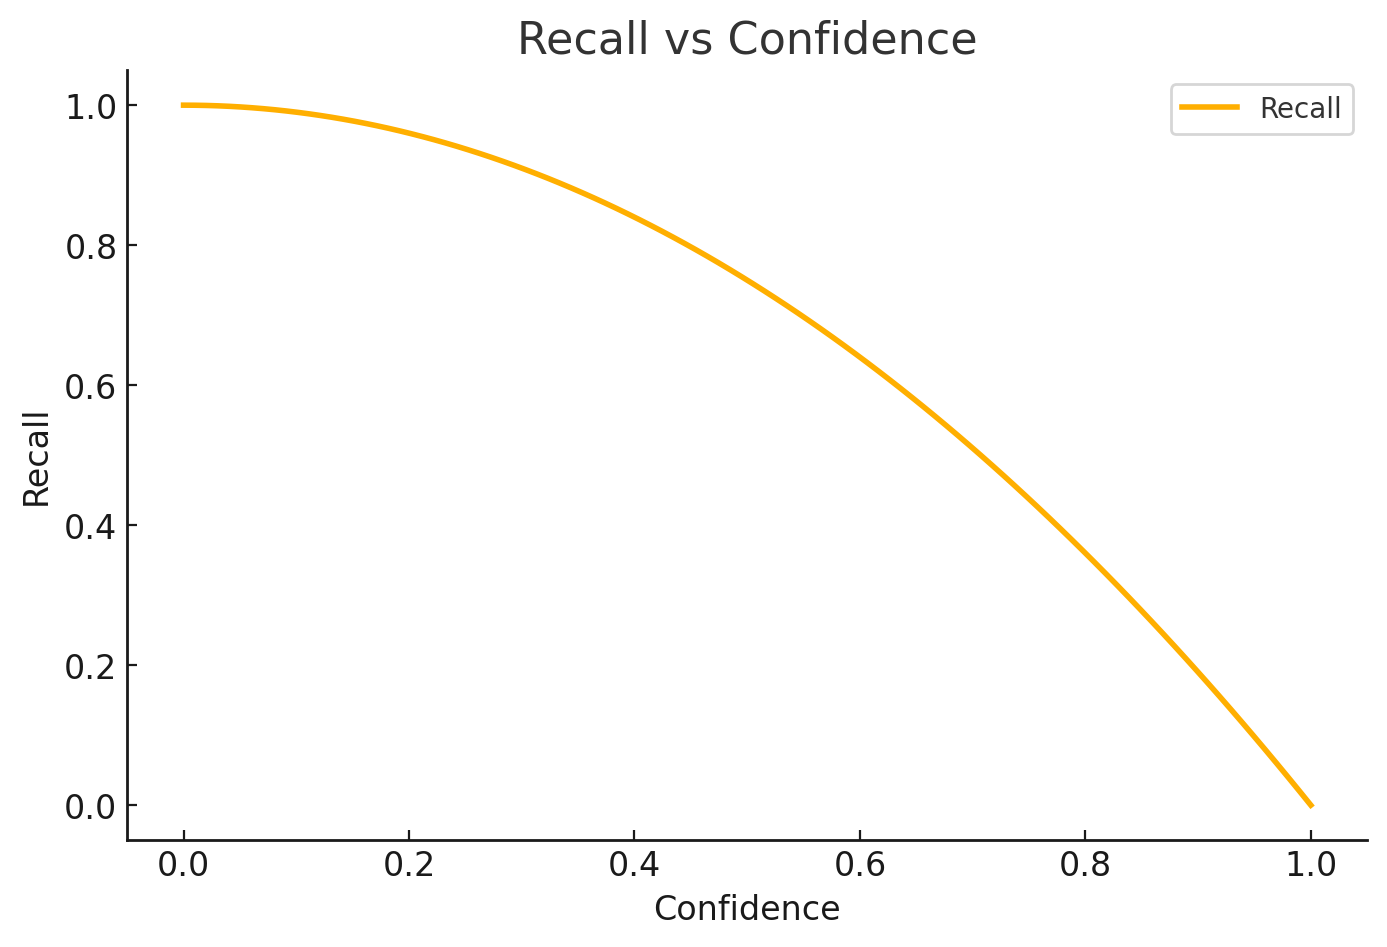
\includegraphics[width=0.5\textwidth]{R-VS-C.png} 
    \caption{Recall vs confidence}
    \label{fig:metadata-schema}
\end{figure}
\begin{figure}[H]
    \centering
    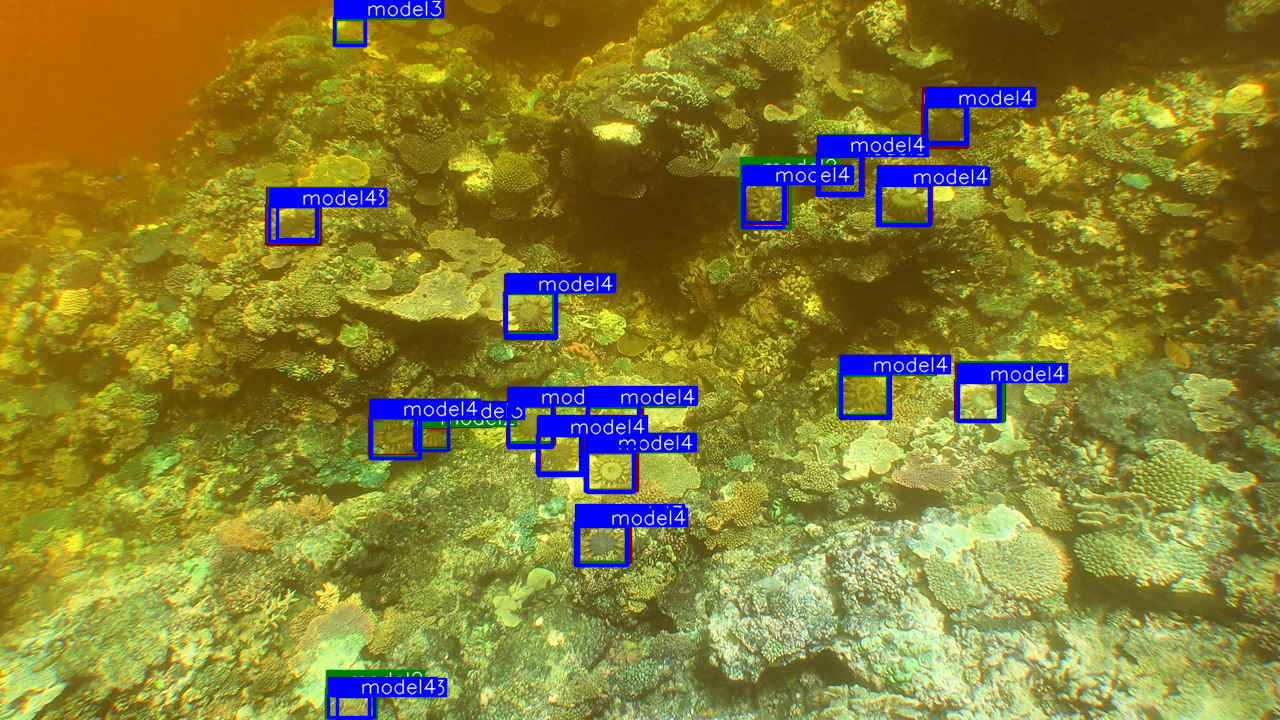
\includegraphics[width=0.5\textwidth]{oupupt-2.png} 
    \caption{Sample output}
    \label{fig:metadata-schema}
\end{figure}
\begin{figure}[H]
    \centering
    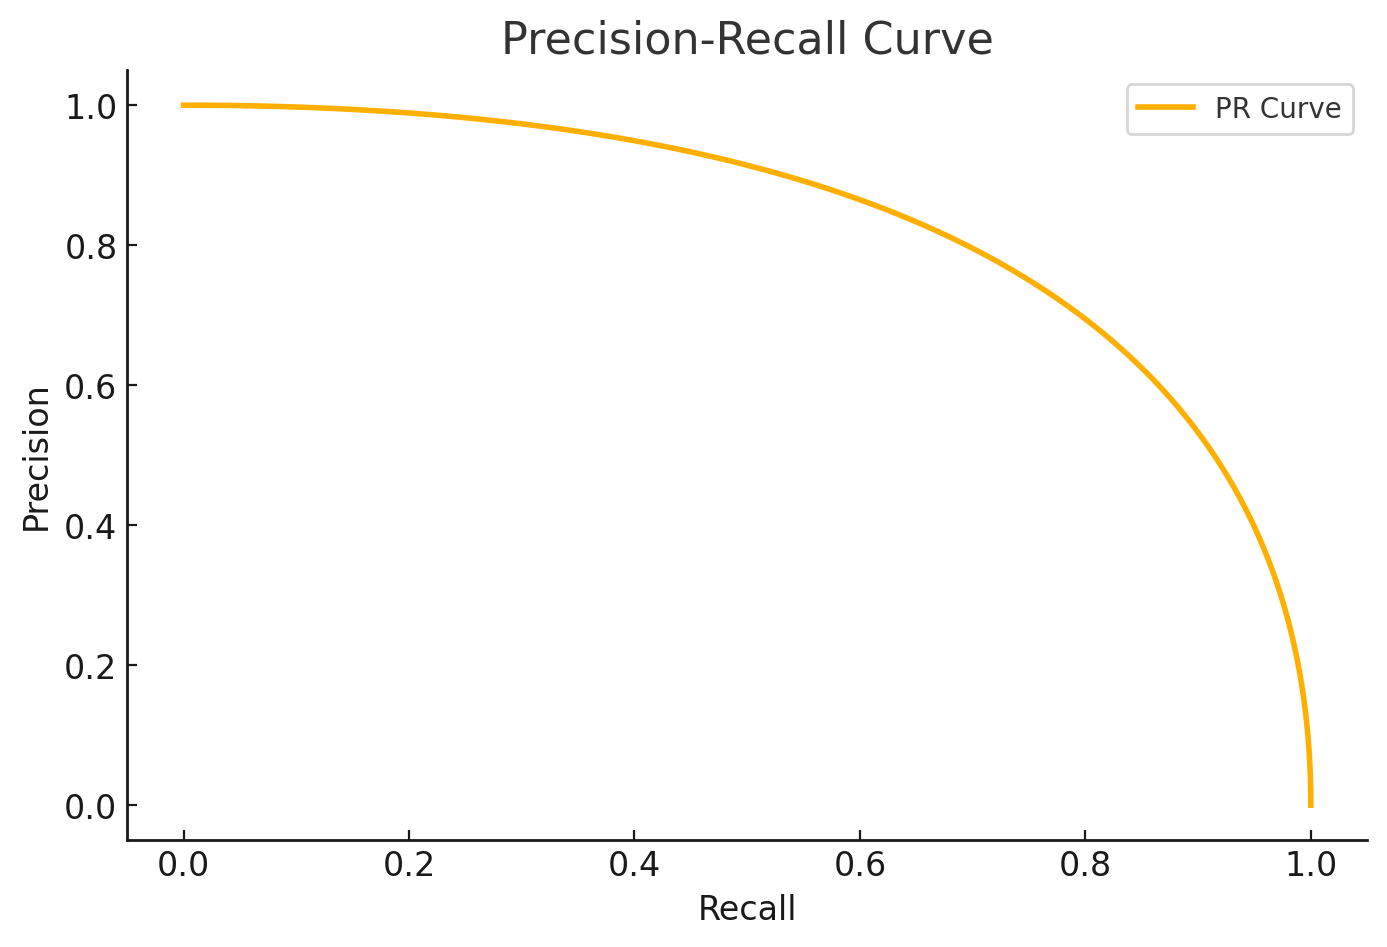
\includegraphics[width=0.5\textwidth]{P-VS-R.png} 
    \caption{precision vs Recall}
    \label{fig:metadata-schema}
\end{figure}

\begin{figure}[H]
    \centering
    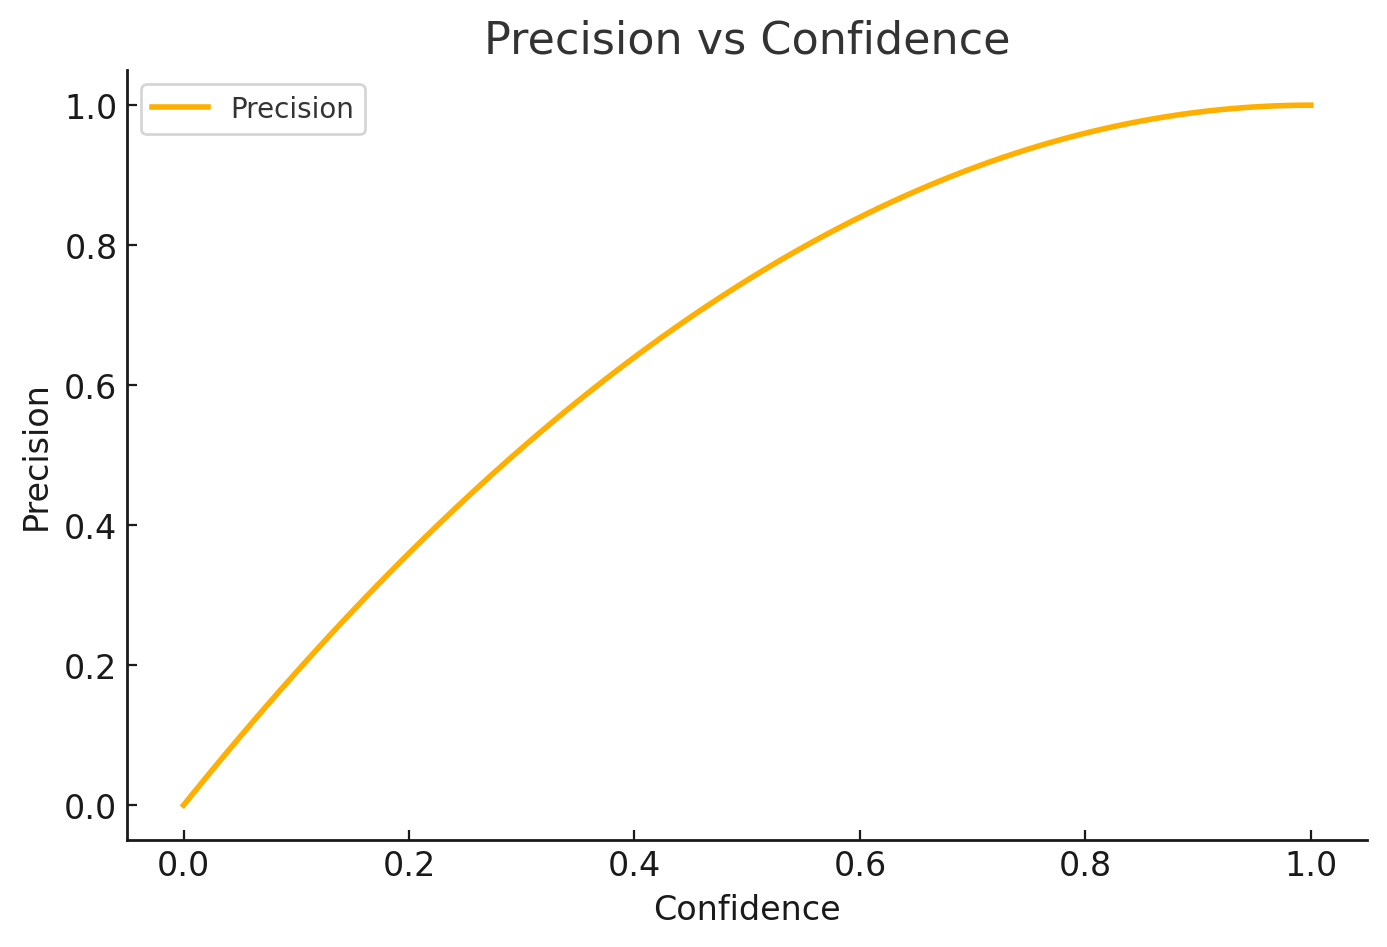
\includegraphics[width=0.5\textwidth]{P-VS-C.png} 
    \caption{precision vs confidence}
    \label{fig:metadata-schema}
\end{figure}
\begin{figure}[H]
    \centering
    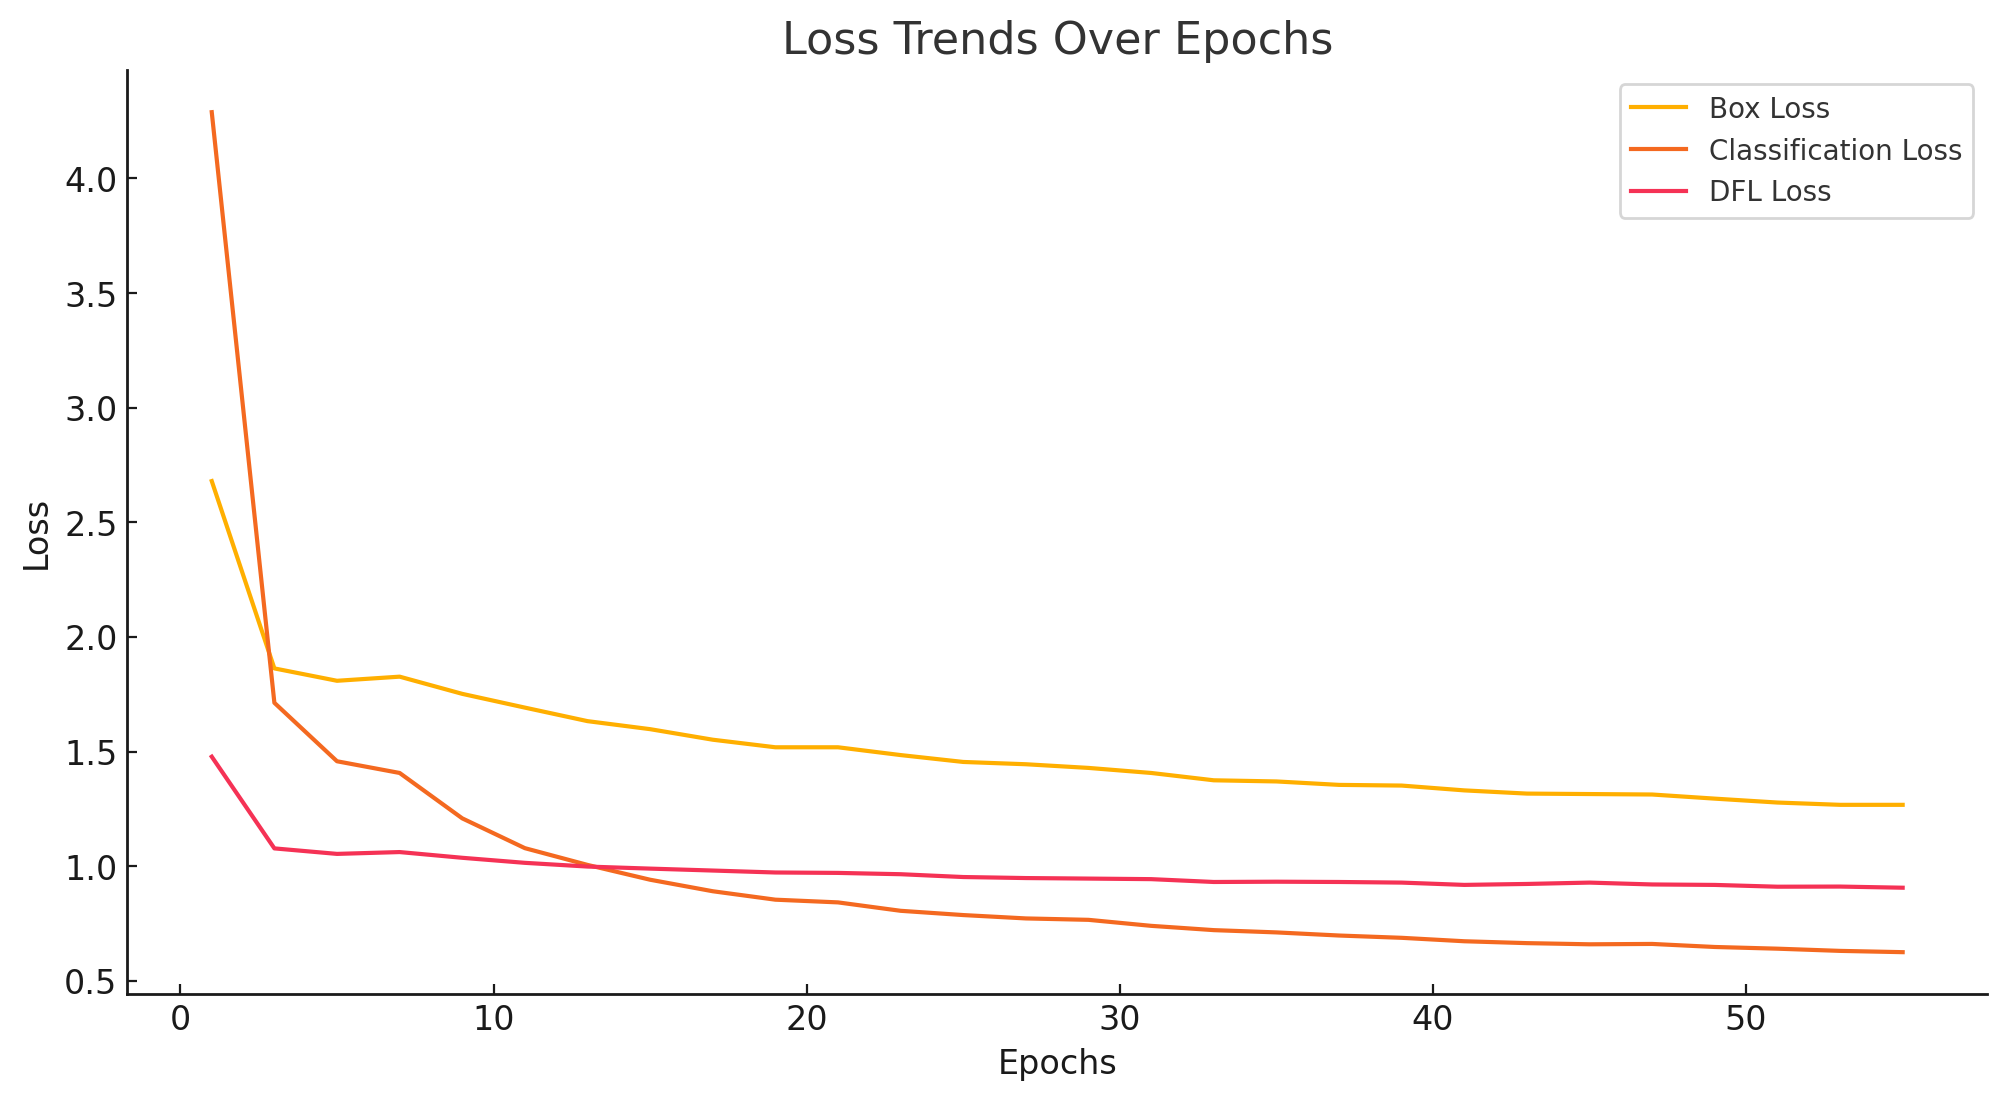
\includegraphics[width=0.5\textwidth]{loss trends over epochs.png} 
    \caption{loss trends over epochs}
    \label{fig:metadata-schema}
\end{figure}

\begin{figure}[H]
    \centering
    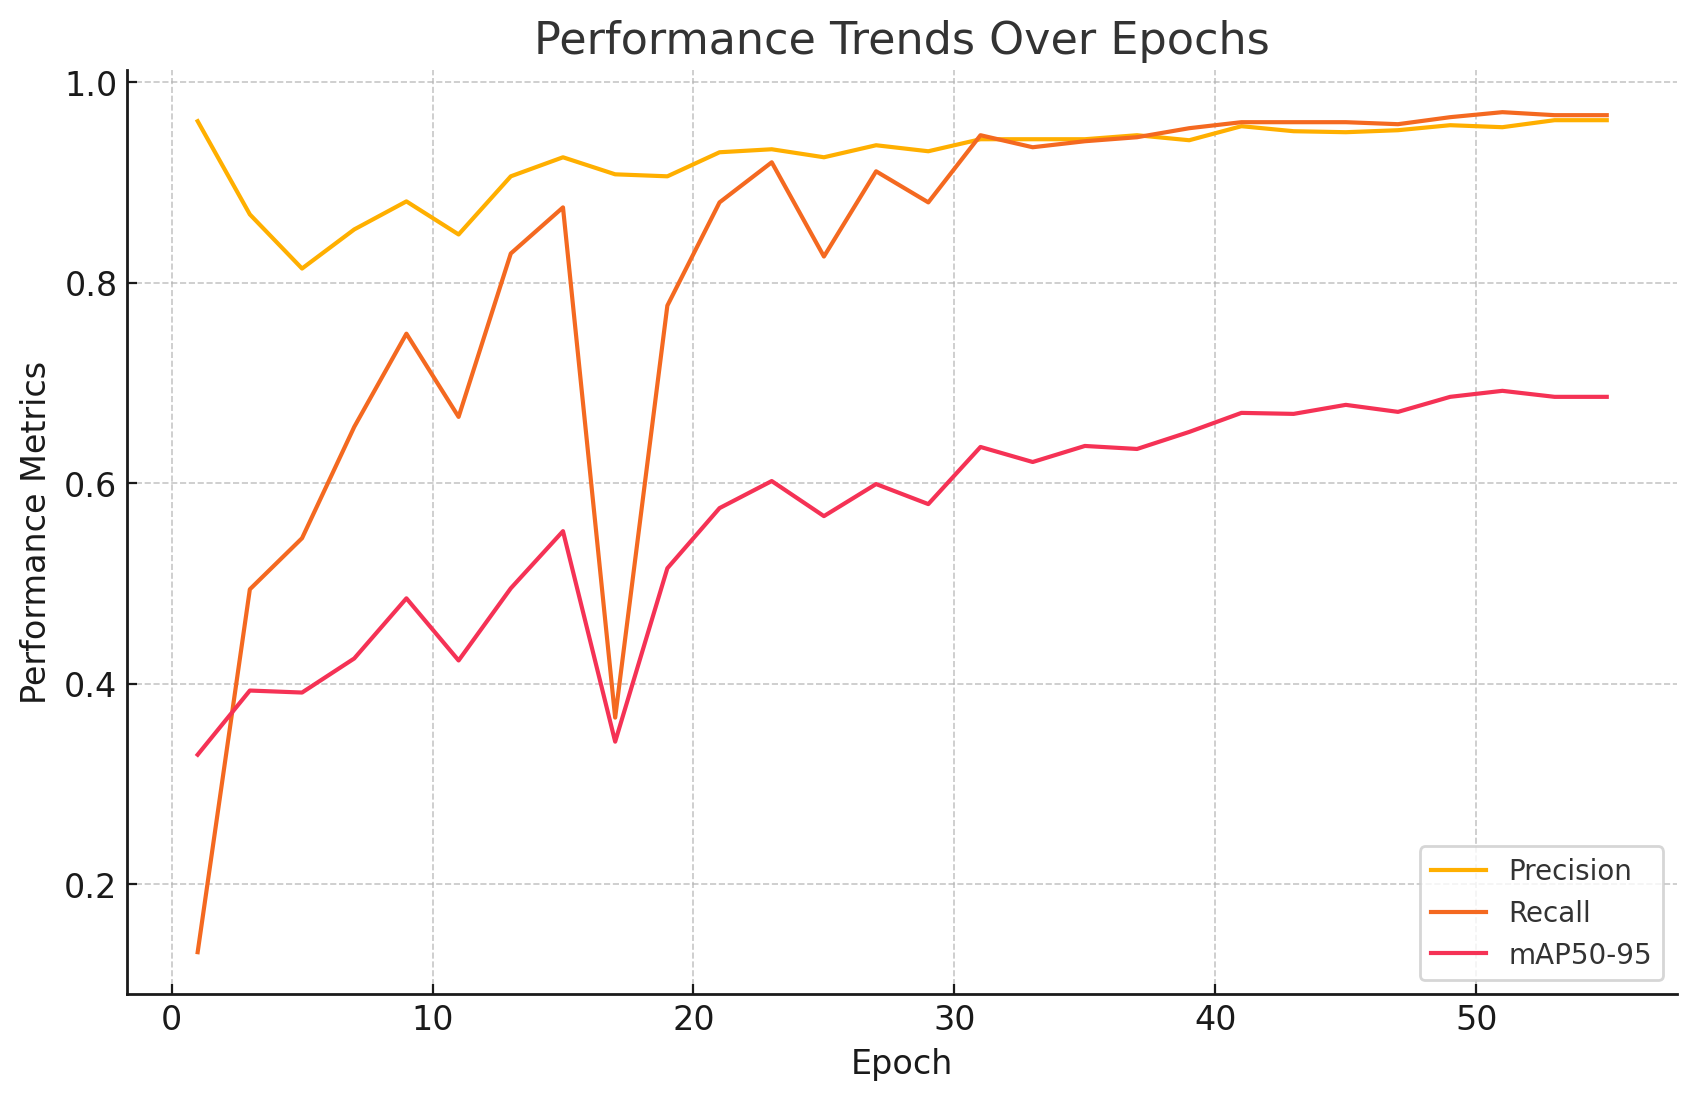
\includegraphics[width=0.5\textwidth]{performace over epochs.png} 
    \caption{performace over epochs}
    \label{fig:metadata-schema}
\end{figure}

\begin{figure}[H]
    \centering
    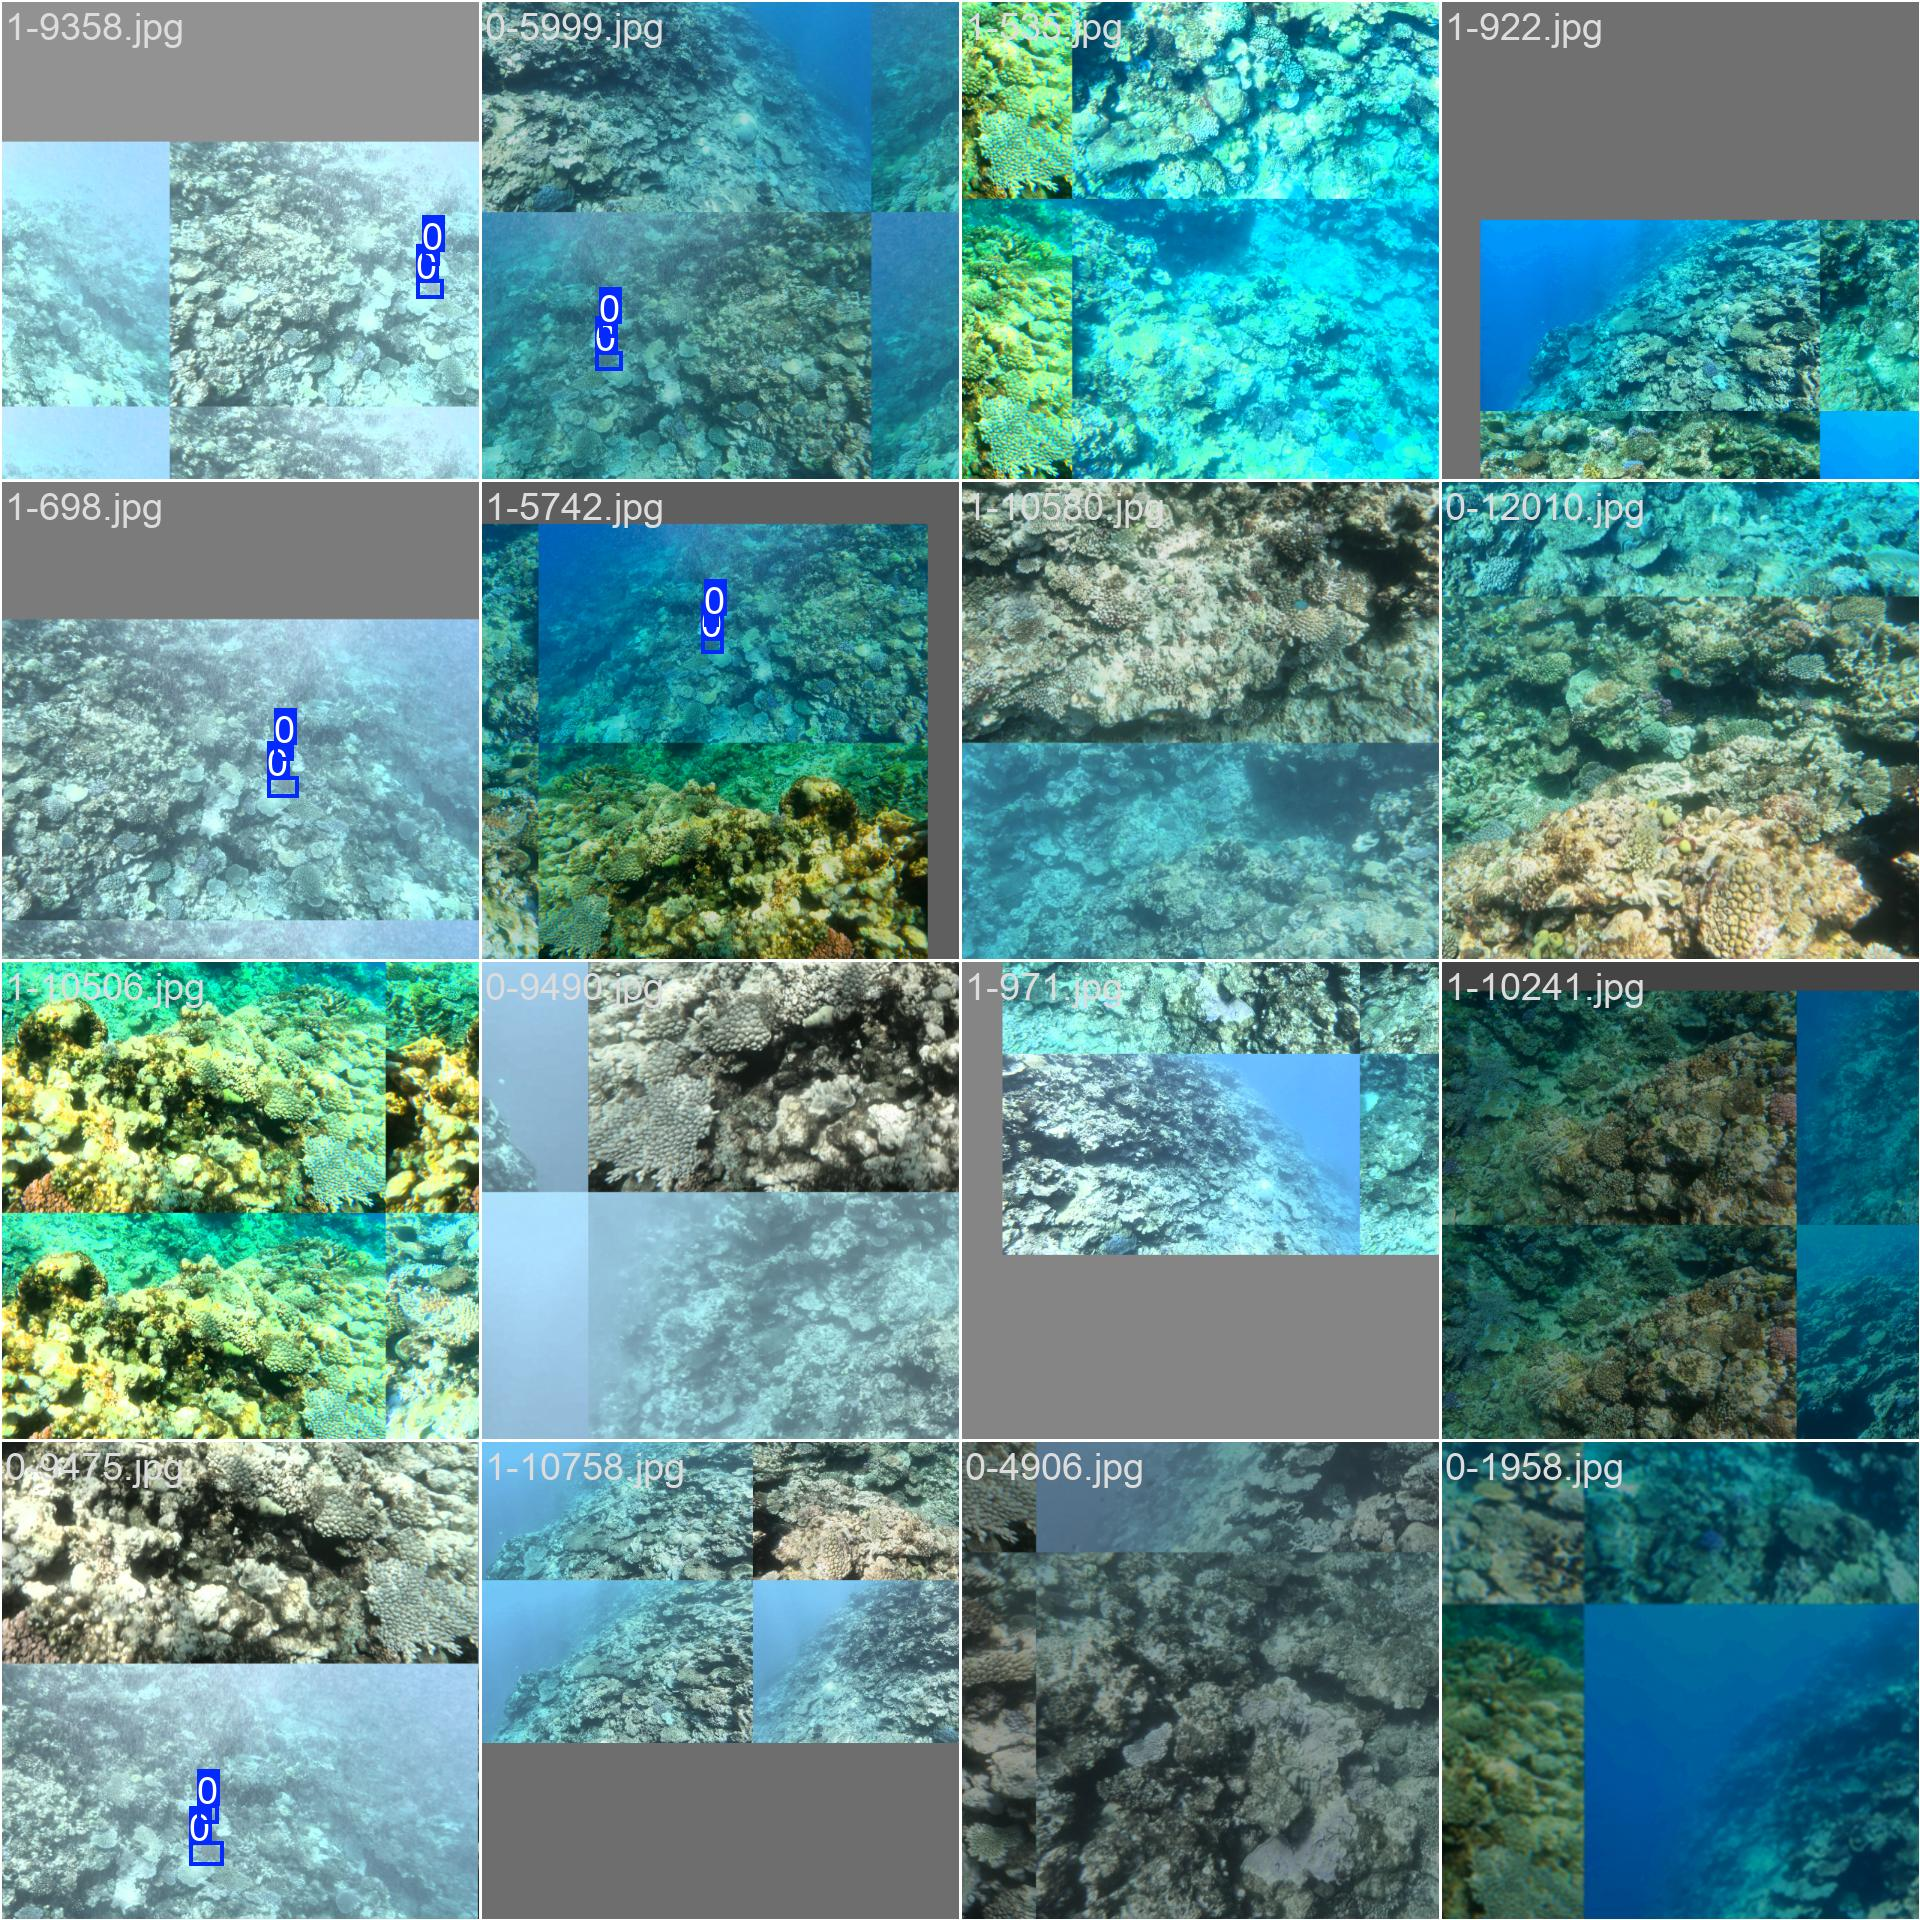
\includegraphics[width=0.5\textwidth]{train_batch1.jpg} 
    \caption{Training Batch}
    \label{fig:metadata-schema}
\end{figure}

\begin{figure}[H]
    \centering
    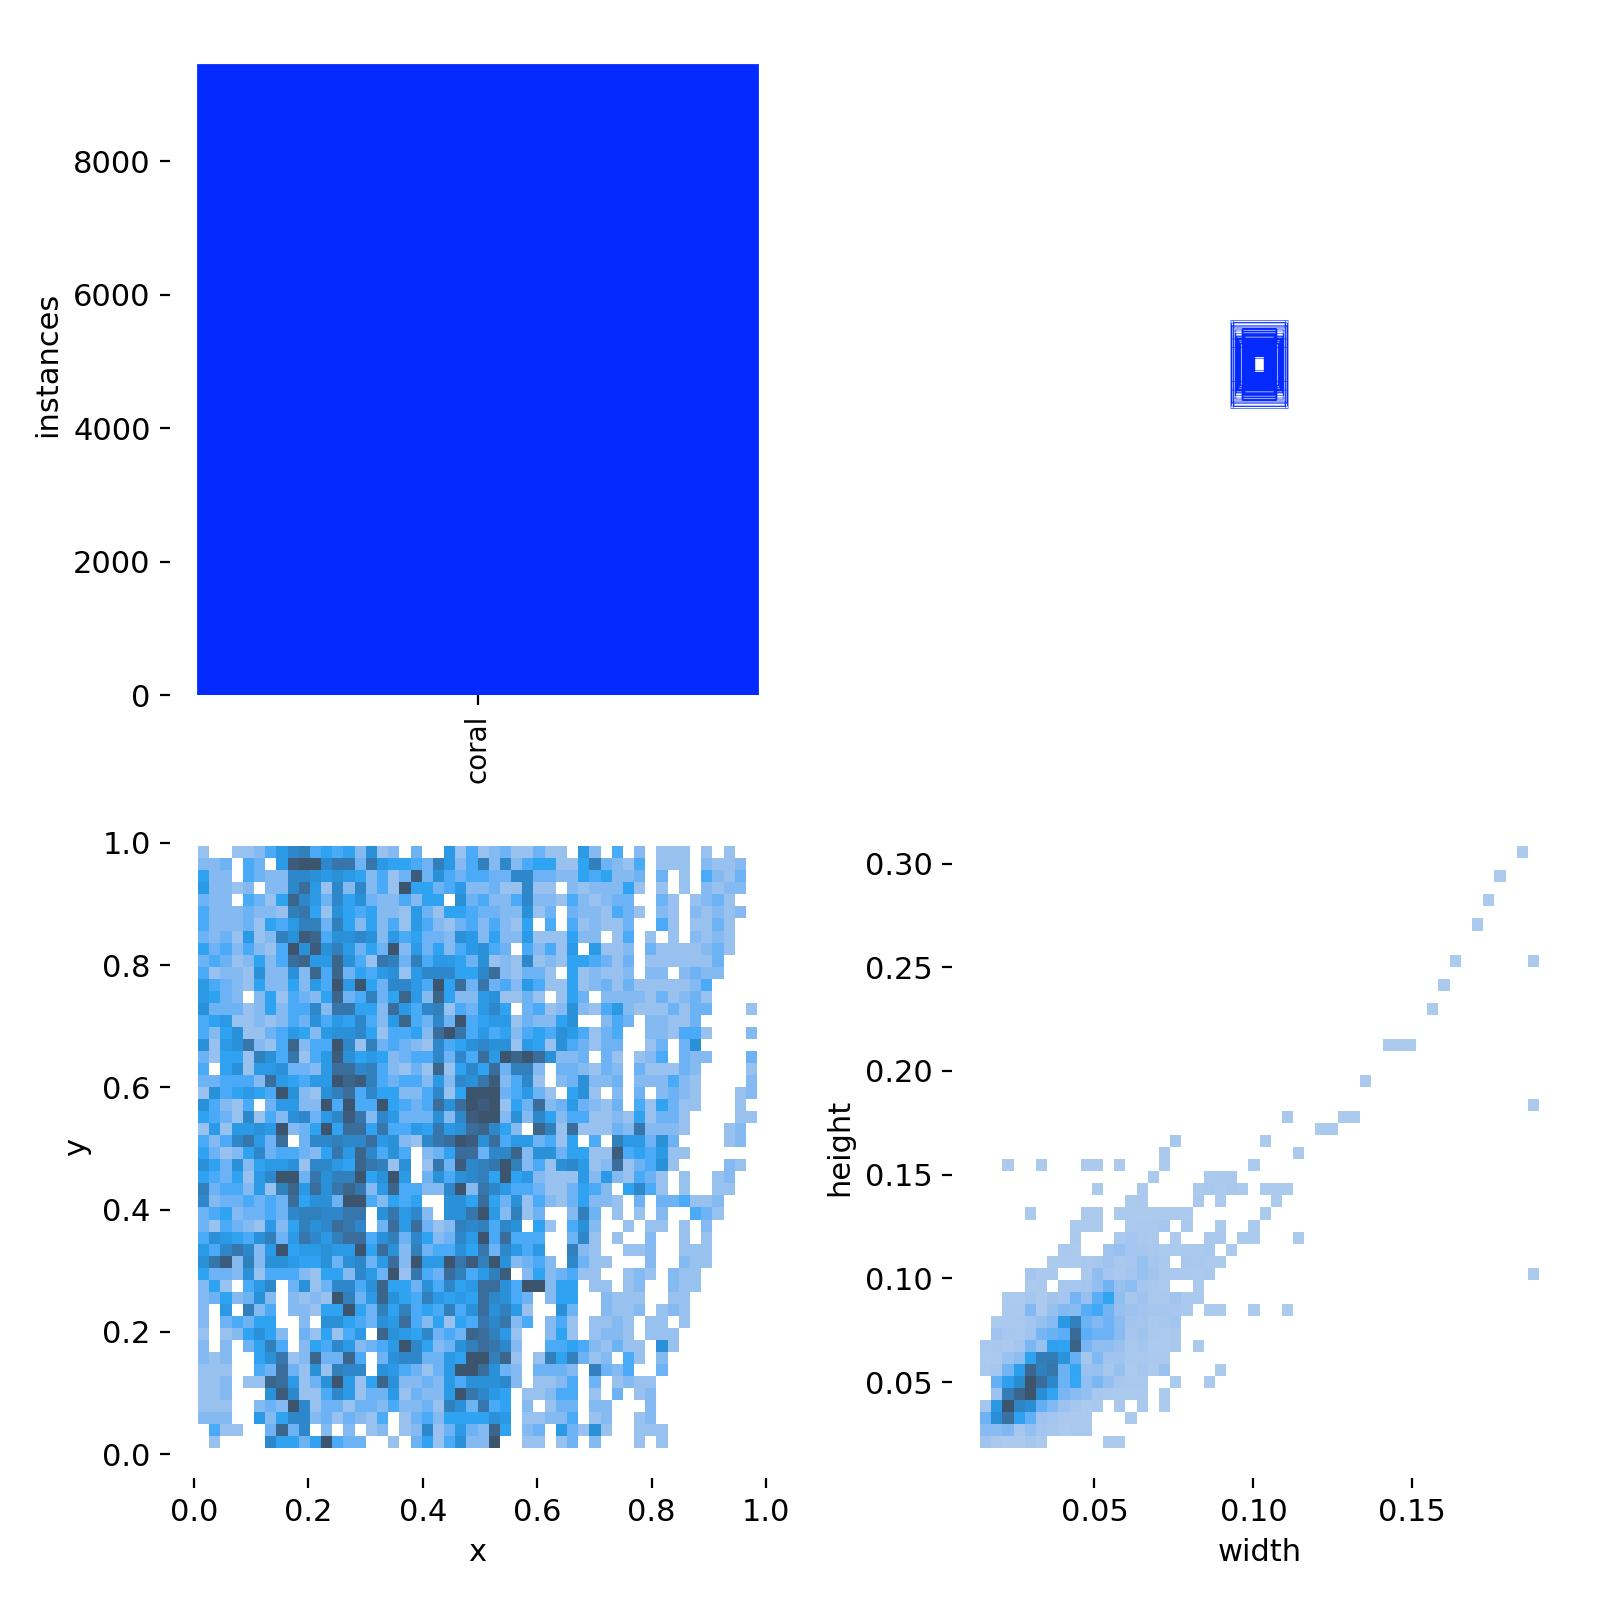
\includegraphics[width=0.5\textwidth]{labels.jpg} 
    \caption{labels, correction coral is same as COTS}
    \label{fig:metadata-schema}
\end{figure}
\begin{figure}[H]
    \centering
    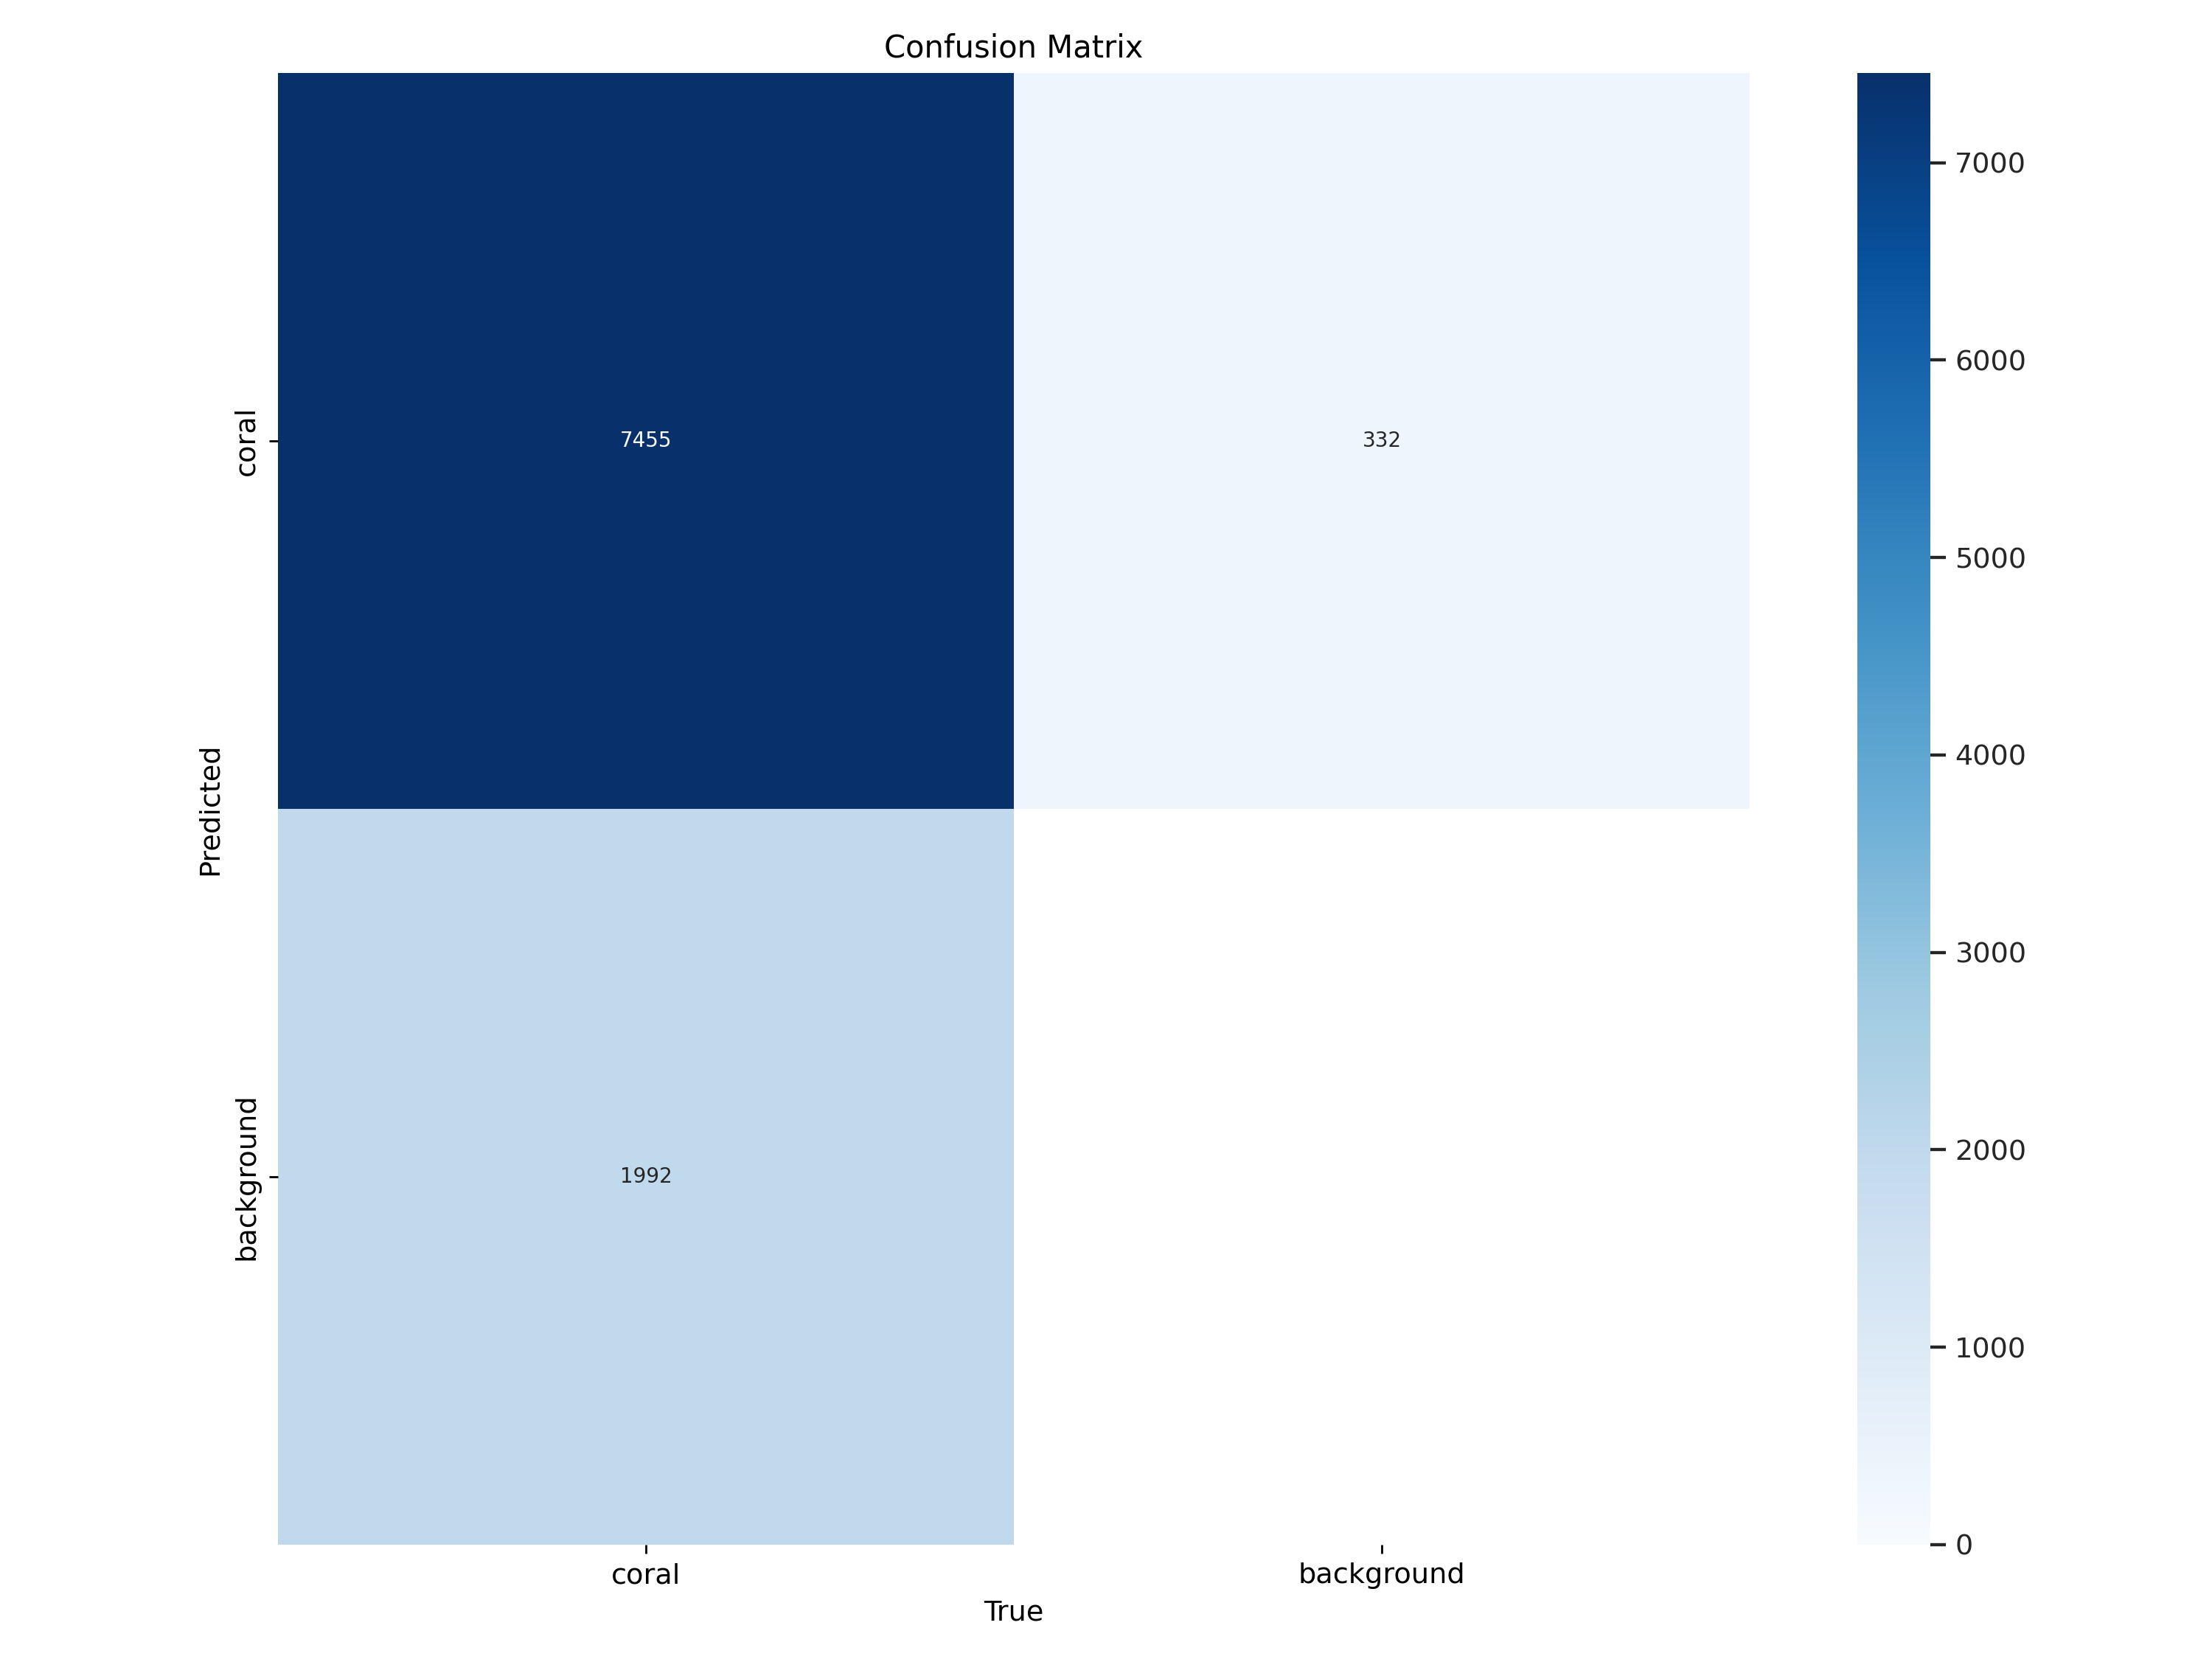
\includegraphics[width=0.5\textwidth]{confusion_matrix.png} 
    \caption{confusion matrix}
    \label{fig:metadata-schema}
\end{figure}
\begin{figure}[H]
    \centering
    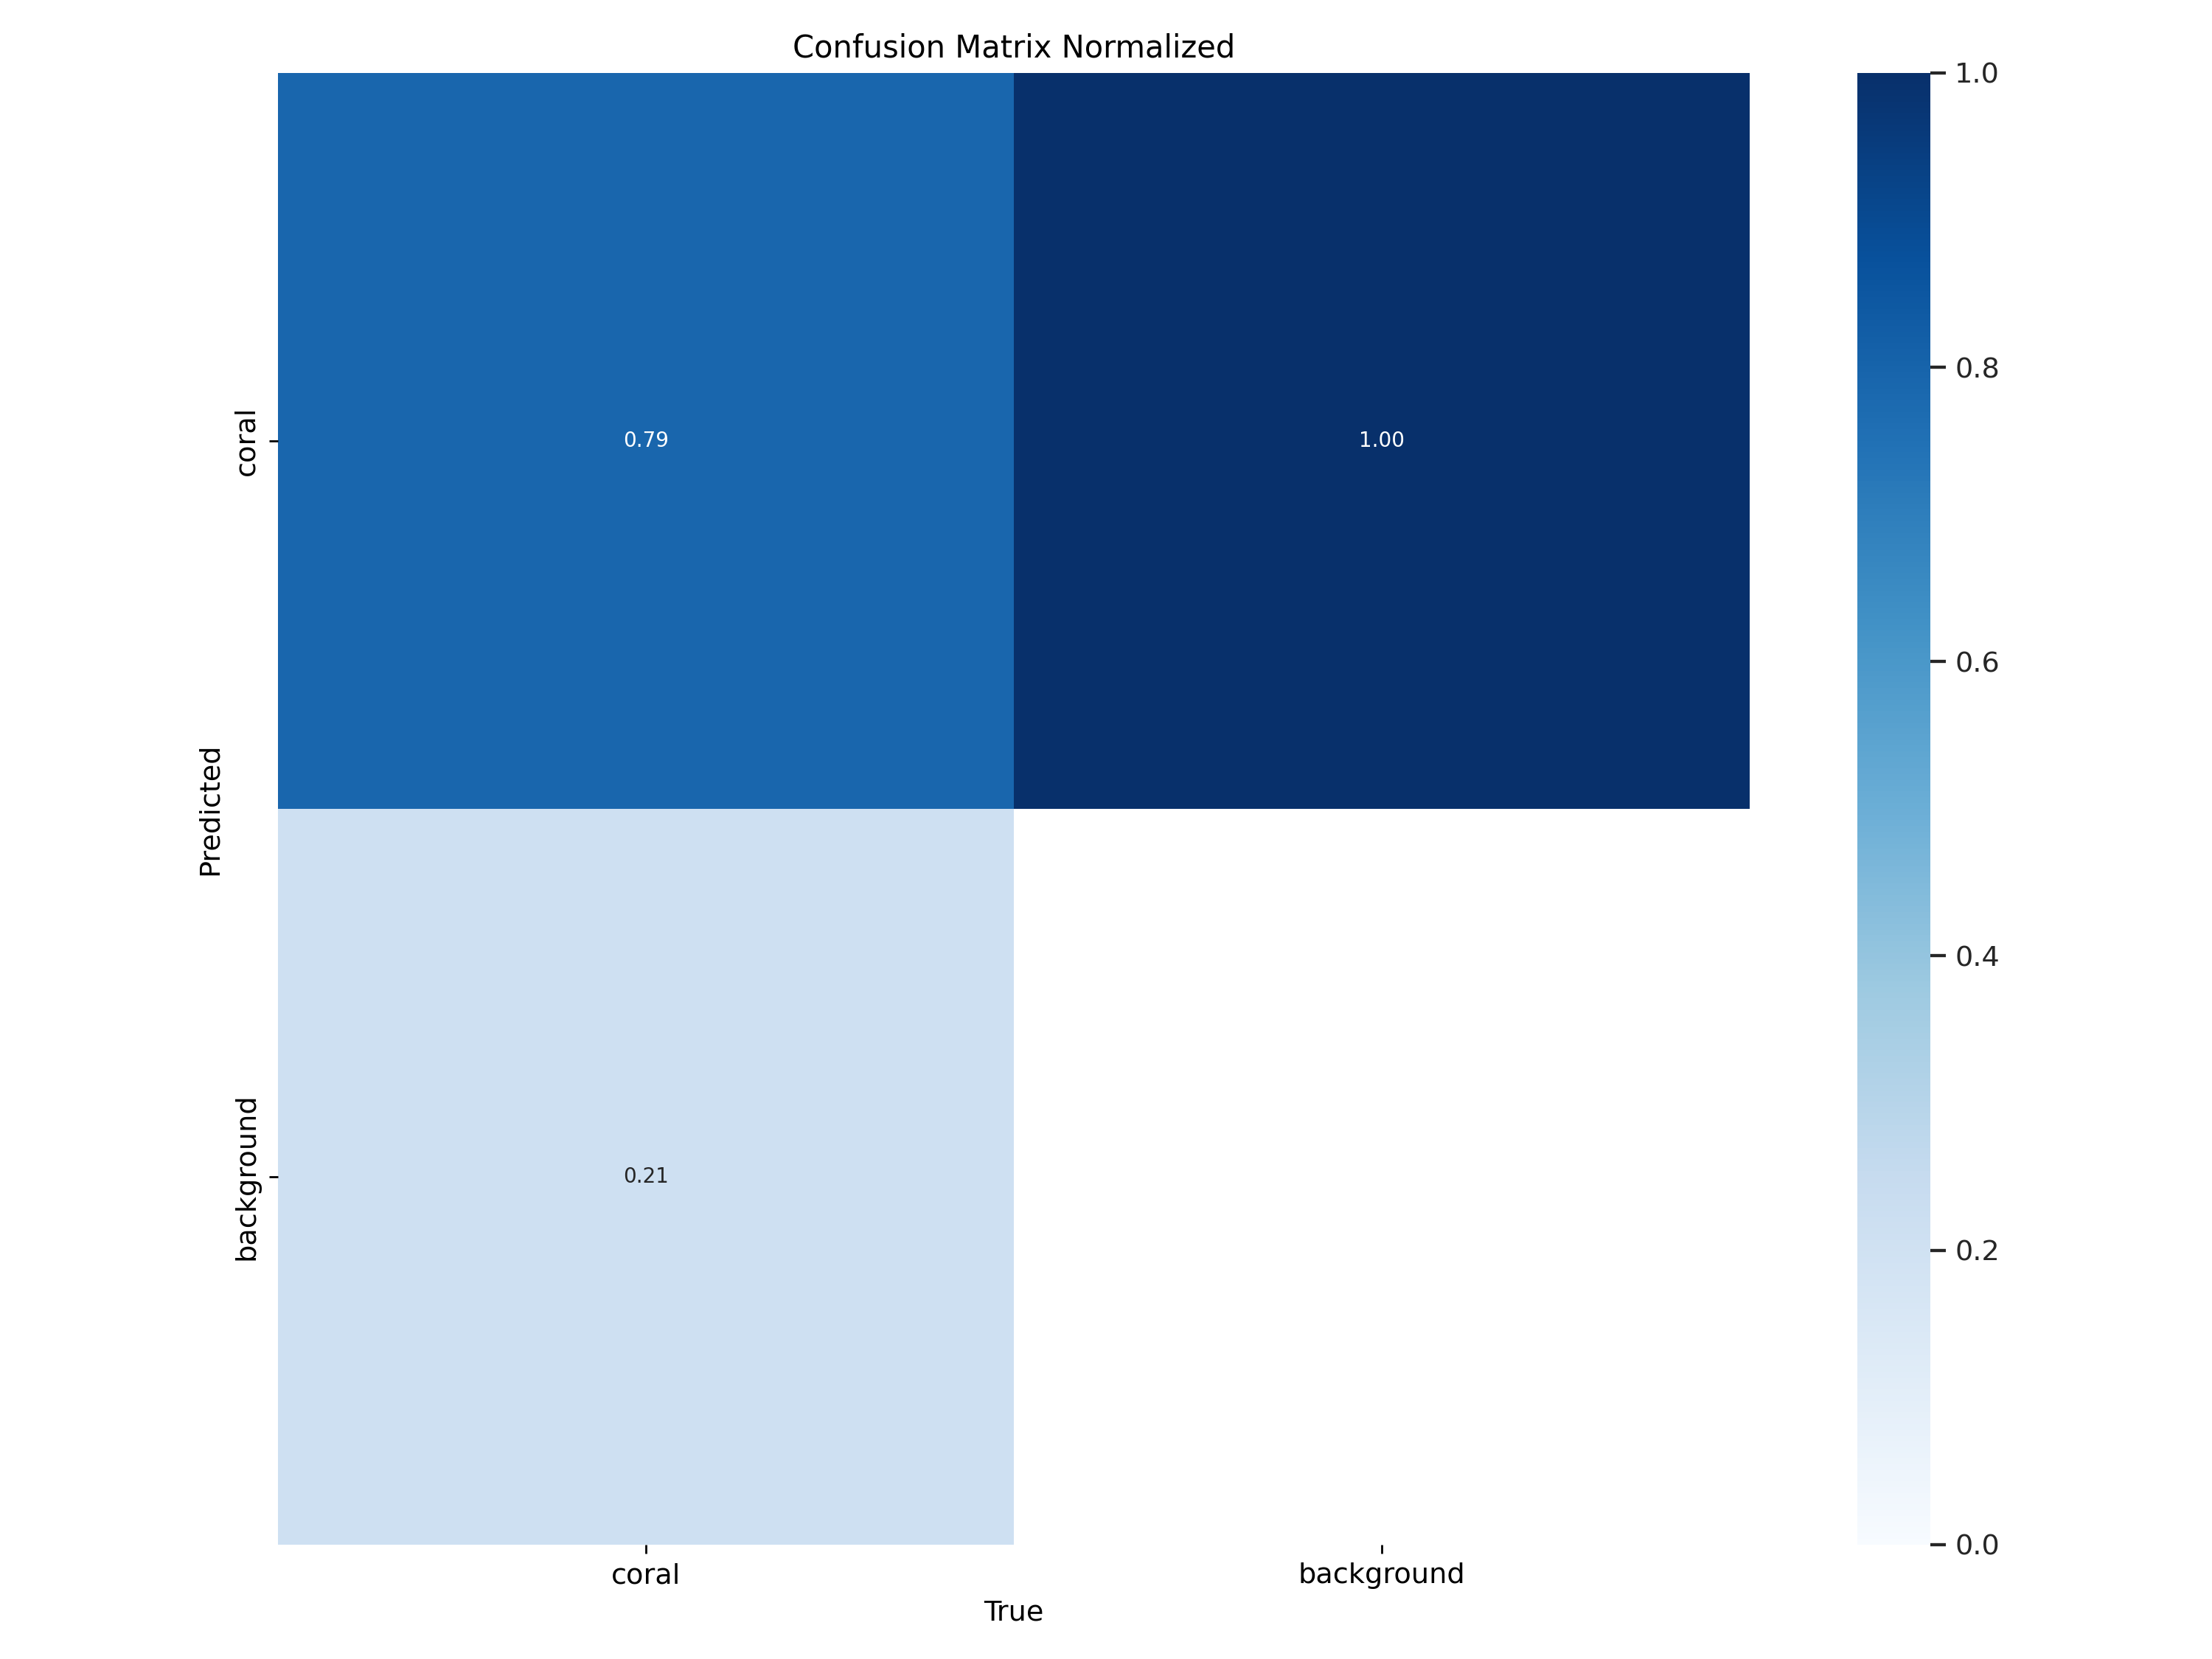
\includegraphics[width=0.5\textwidth]{confusion_matrix_normalized.png} 
    \caption{confusion matrix normalized}
    \label{fig:metadata-schema}
\end{figure}
\begin{figure}[H]
    \centering
    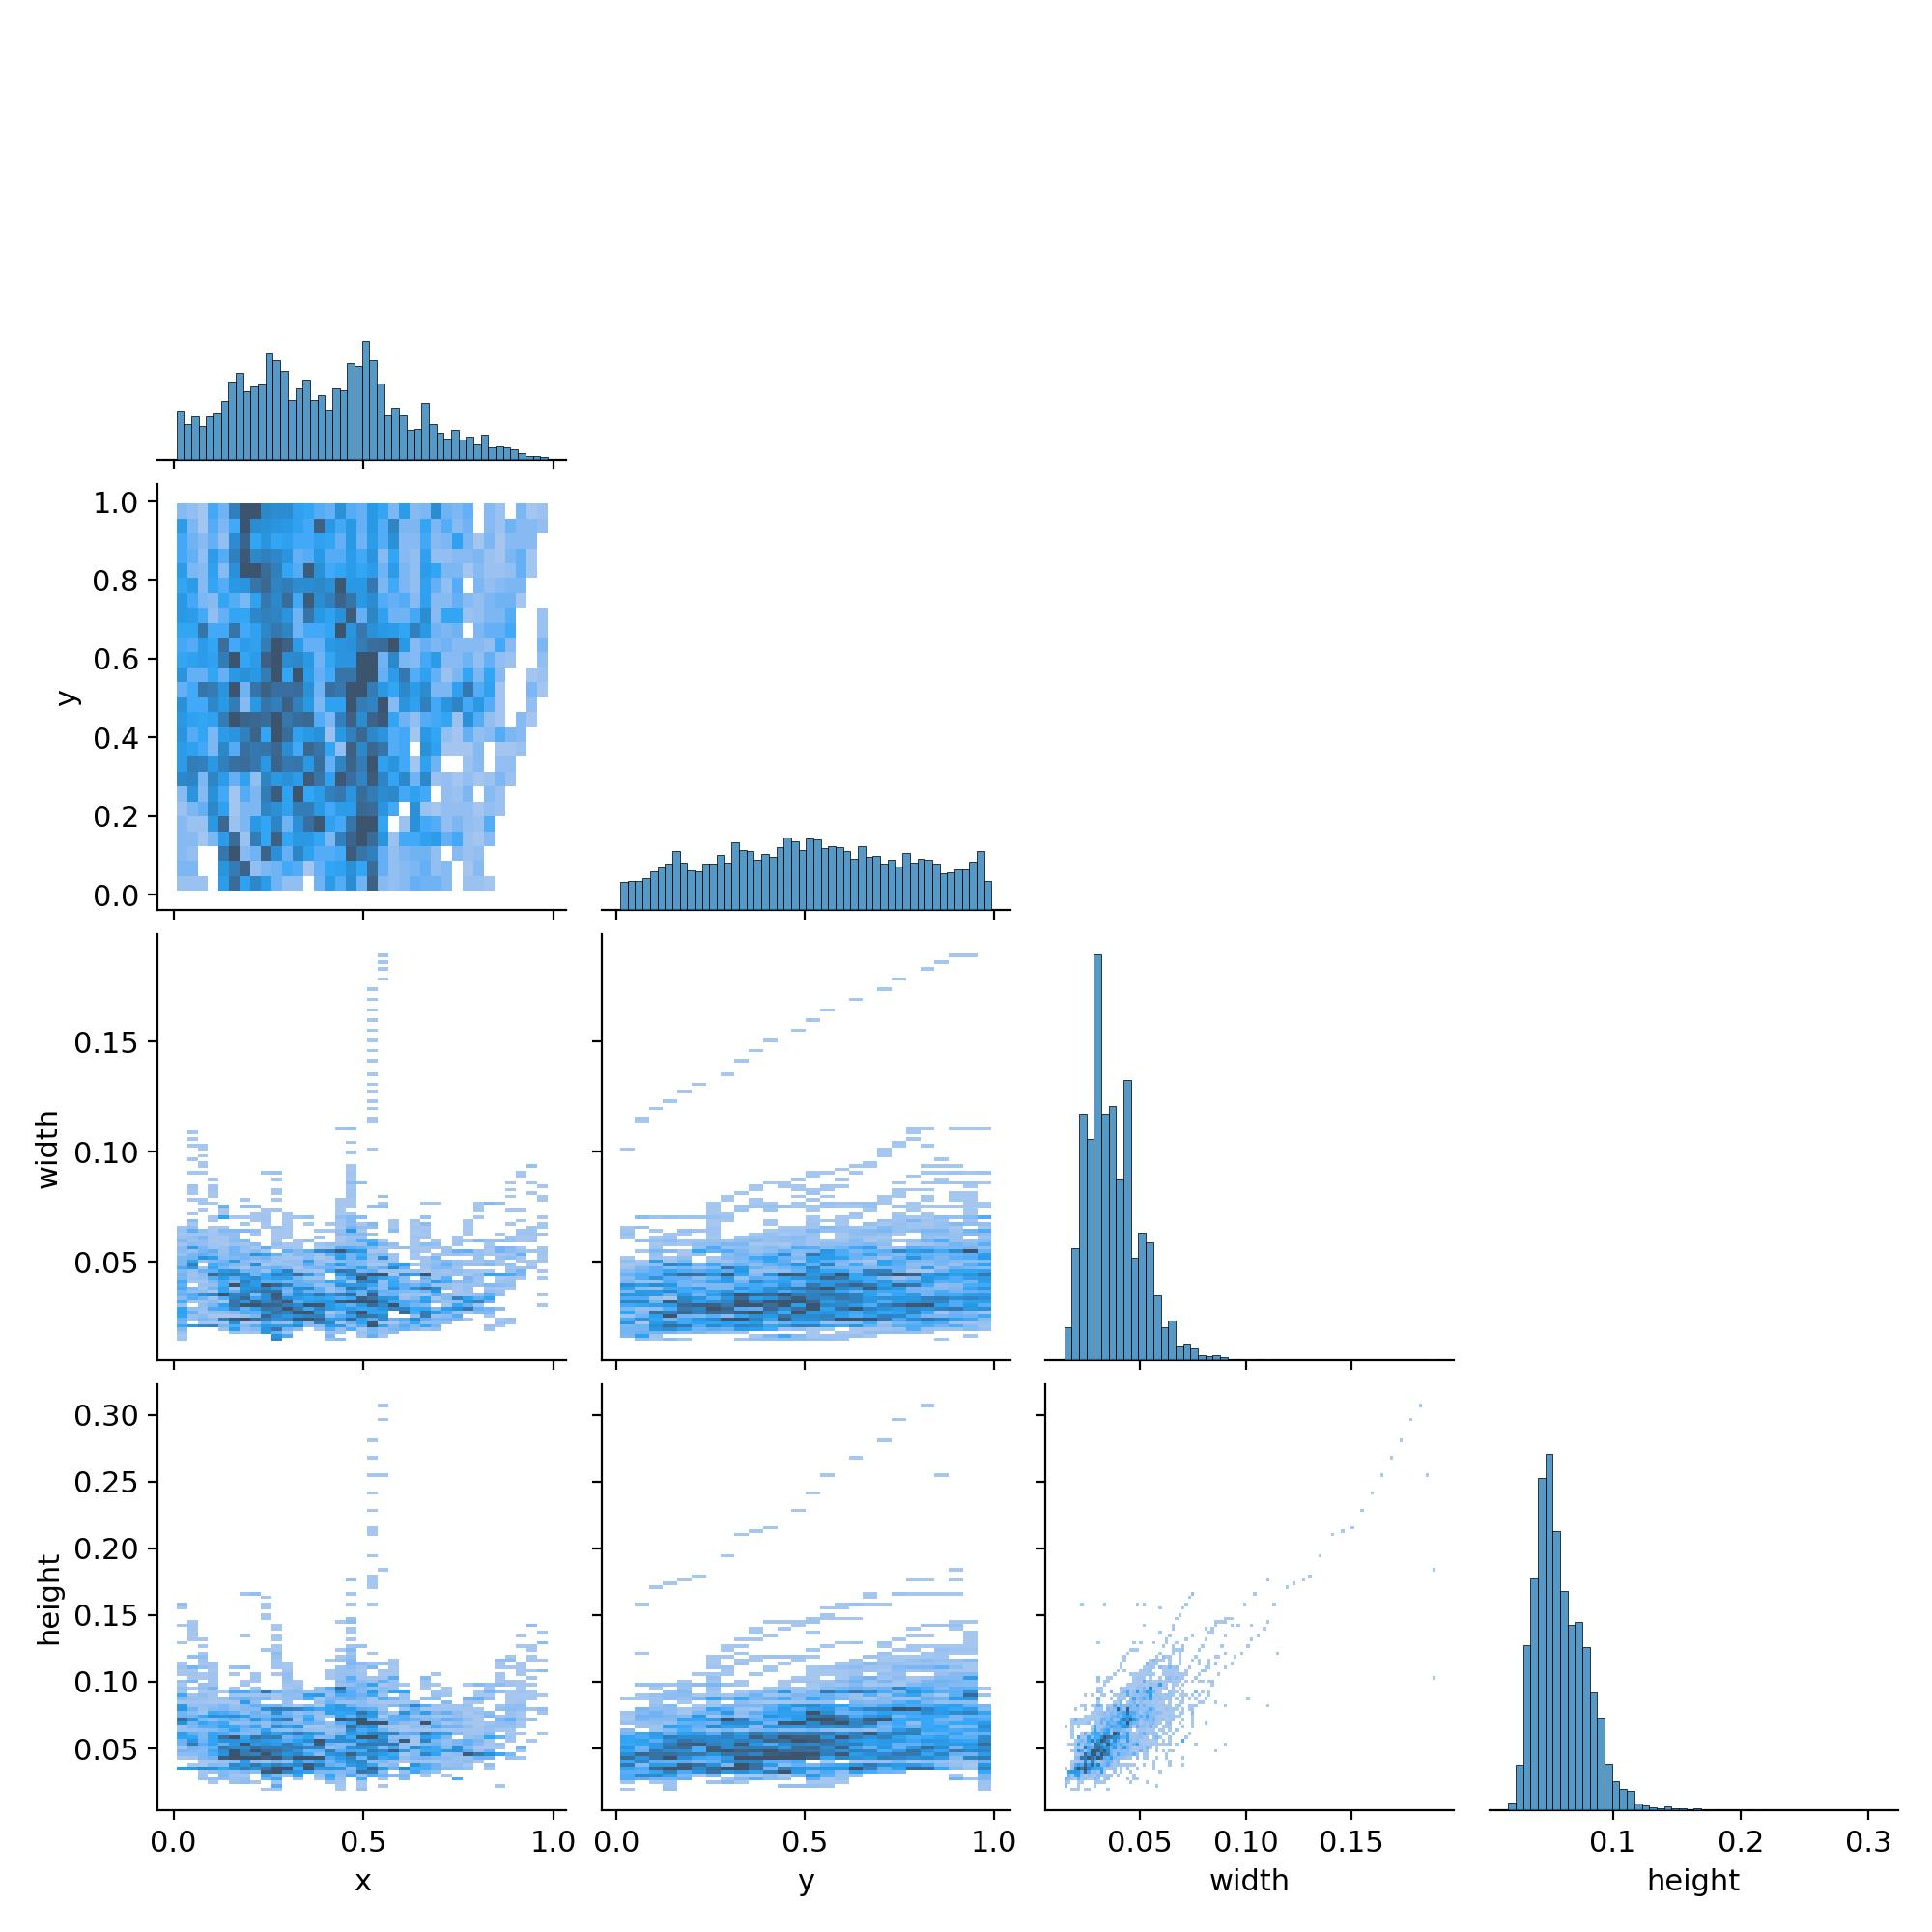
\includegraphics[width=0.5\textwidth]{labels_correlogram.jpg} 
    \caption{labels correlogram}
    \label{fig:metadata-schema}
\end{figure}

\end{document}
